\documentclass[11pt]{article}

% Camera-ready mid-project report: show author names.
\usepackage[final]{acl}

\usepackage{times}
\usepackage{latexsym}
\usepackage[T1]{fontenc}
\usepackage[utf8]{inputenc}
\usepackage{microtype}
\usepackage{inconsolata}
\usepackage{graphicx}
\usepackage{booktabs}
\usepackage{amsmath}
\usepackage{amssymb}
\usepackage{enumitem}
\usepackage{url}
\usepackage{caption}

\title{GraphModi: Updating Graph Language Models in Multi-turn Dialogue\\
\large Mid-Project Progress Report}

\author{
  Prasoon Dev\quad
  Yajat Lakhanpal\quad
  Hrishiraj Mitra\quad
  Arihant Rastogi \\
  Team Hansraj \\
  International Institute of Information Technology, Hyderabad
}

\begin{document}
\maketitle

\begin{abstract}
Graph language models (GLMs) answer questions from soft graph tokens, where the graph is assumed to be fixed.
In dialogue, users revise the world, and thus, the graph tokens computed before become stale.
We build a synthetic benchmark of multi-turn sessions (4,455 turns per split), where each turn is an update followed by a question and 41\% of test turns change the answer.
GraphModi (our proposed solution) converts each revision into a typed edit program, applies it to an explicit graph, re-encodes the result, and answers from the new graph tokens with a frozen Llama-3.1-8B-Instruct, never seeing the revision text.
Overall on test, re-encoding the correct graph has TEA (35.1\%) and GraphToken (37.9\%) model, against 32.5\% and 33.3\% with stale tokens plus the revision text, 29.8\% and 29.6\% when the graph is encoded only once, and 27.7\% with no graph; a soft prompt that reads the revision text scores 34.2\%. These results motivate the need of such a framework which allows a GLM to re-encode its own input for maintaining correct chat history and updates. 
\end{abstract}

\section{Introduction}
\label{sec:intro}

Graph language models (GLMs) map a graph through a GNN into soft tokens that a frozen or adapted language model can attend to~\cite{perozzi2024graphtoken,wang2024teaglm,he2024gretriever,plenz-frank-2024-graph}.
All such work assumes the graph does not change.
Real graphs face updates as a user may report real time updates.
After such a change, graph tokens computed from the old graph describe a world that no longer exists.

One way to fix this is by keeping updates in the text context and rely on the language model to track these.
Dynamic-graph QA benchmarks study this setting with graphs described in text~\cite{comrie2025dygraphqa}.
Another is to update stored knowledge directly, but parametric knowledge editors can recall a new fact and fail to propagate its effects~\cite{zhong-etal-2023-mquake}.
GraphModi keeps state external: an edit program is applied to an explicit graph, the graph is re-encoded, and the QA call receives only the new graph tokens and the question, never the updation text.
This lets us score writing (did the edit land?) separately from reading (can the model answer from the new tokens?).

\paragraph{Research questions.}
\begin{description}[leftmargin=0.5em,style=nextline,font=\normalfont\itshape,itemsep=1pt]
  \item RQ1 : Can a frozen LLM emit executable edit programs from a few-shot prompt, and what do its errors cost downstream?
  \item RQ2 : Does answering from re-encoded tokens beat stale $G_0$ tokens and text-history controls as turns accumulate, especially on answer-changing turns?
  \item RQ3 : Do graph tokens carry information beyond graph-blind baselines?
\end{description}

\paragraph{Contributions.}
To answer the above questions, we provide the contributions using our project
\begin{description}[leftmargin=0.5em,style=nextline,font=\normalfont\itshape,itemsep=1pt]
  \item i) A formulation of multi-turn GLM updating with an edit language and executor. This separates write accuracy from read accuracy.
  \item ii) A multi-turn evaluation grid across graph size, density, session length, and task, with paired conditions that isolate stale tokens, text history, and graph-blind controls.
  \item iii) Evidence that stale graph tokens degrade over turns and that re-encoding helps most on turns where an edit would change the answer.
\end{description}

\section{Related Work}
\label{sec:lit}

\paragraph{Graphs as text.}
We represent a graph in natural language. This enables an LLM to attempt structural reasoning on the with no GNN~\cite{wang2023nlgraph,fatemi2024talk}.
\citet{fatemi2024talk} shows that accuracy varies substantially with how the graph is encoded as text, and \citet{wang2023nlgraph} finds that LLM graph reasoning can break when it relies on irrelevant patterns instead of the actual relationships in the graph
Many of our controls use text history, so these results set the baseline a GLM has to beat.

\paragraph{Soft graph tokens.}
GraphToken learns a graph encoder end-to-end through the language-modelling objective~\cite{perozzi2024graphtoken}.
TEA-GLM pretrains a GNN, aligns it with the LLM's token embeddings, freezes it, and then trains a linear projector onto a fixed number of tokens~\cite{wang2024teaglm}.
G-Retriever and the graph language models of \citet{plenz-frank-2024-graph} also couple graph representations with frozen or lightly adapted LMs~\cite{he2024gretriever}.
All of them evaluate QA against a graph supplied once per query and do not explore how a query based revision should modify the encoded graph.
We build TEA-style and GraphToken-style variants rather than claim exact reproductions, since our readouts, tasks, and training data differ from the originals.

\paragraph{Do GLMs use the graph?}
CLEGR shows that a graph-blind soft-prompted LLM can rival full GLMs on metro reasoning, and proposes a shuffled-graph control to detect this~\cite{petkar2026clegr}.
\citet{liu2024softpromptgraph} ask the same question for soft prompting on graph learning tasks.
We adopt the soft-prompt baseline and the shuffled-graph control, and treat parity with either as evidence against a graph-reading claim.

\paragraph{Dynamic graphs and stateful dialogue.}
DyGraphQA evaluates LLMs on graphs that change through additions and deletions described as text or structured data~\cite{comrie2025dygraphqa}.
MQuAKE shows that knowledge edits made inside model parameters often fail to propagate to multi-hop questions~\cite{zhong-etal-2023-mquake}.
SKG-Eval stores conversational claims in an incremental knowledge graph to detect cross-turn conflicts~\cite{shil2026skgeval}.

\section{Problem Formulation}
\label{sec:problem}

Consider a transit assistant that initially knows two routes between a pair of stations.
The user then says that one station is closed.
The text decoder sees the correction, but a frozen graph representation still describes the station as open.
The model is now given two versions of the world.
Keeping the full conversation in the prompt may help, but it does not repair the graph that the GNN encodes.
It can also make the system depend on implicit state tracking by the language model.
This needs \emph{writing} (mapping a revision to a graph change) and \emph{reading} (answering from re-computed graph tokens), which we score separately on turns when the edit changes the answer and when it does not.

Therefore, we formalize the problem as follows.

\paragraph{Graph and session.}
Let $G=(V,E,a,\rho)$ be an undirected attributed metro graph.
Node attributes include line, accessibility, and $\mathrm{status}\in\{\mathrm{open},\mathrm{closed}\}$; edge relations $\rho$ are $\mathrm{track}$ or $\mathrm{transfer}$.
A session is $S=(G_0,(r_t,q_t)_{t=1}^{T})$, where $r_t$ is a natural-language revision and $q_t$ a question.

\paragraph{Edit language.}
An edit program is a semicolon-separated list of at most three operations terminated by \texttt{END}.
Legal operators are \texttt{SET NODE} (toggle station status), \texttt{ADD EDGE}, \texttt{DEL EDGE}, and \texttt{NOOP}.
Gold programs $P_t^\star$ induce
\begin{equation}
G_t=\mathrm{Apply}(G_{t-1},P_t^\star).
\end{equation}
Gold and stale answers are $a_t^\star=\mathrm{Solve}(G_t,q_t)$ and $\tilde{a}_t=\mathrm{Solve}(G_{t-1},q_t)$; the answer-changing set is $\mathcal{C}=\{t:a_t^\star\neq\tilde{a}_t\}$.

\paragraph{GraphModi.}
At each turn the system computes
\begin{align}
\hat{P}_t &= f_{\mathrm{edit}}(r_t), \\
\hat{G}_t &= \mathrm{Apply}(\hat{G}_{t-1},\hat{P}_t), \\
Z_t &= W\cdot\rho\bigl(\mathrm{GNN}(X(\hat{G}_t)),q_t\bigr)\in\mathbb{R}^{K\times d}, \\
\hat{a}_t &= \mathrm{LLM}\bigl(\mathrm{prompt}(q_t),\,Z_t\bigr).
\end{align}
Edit prediction uses the revision text only; the graph is used for node name resolution.
The revision $r_t$ is withheld from the QA call, so a correct answer after an edit will come from the updated tokens.
The LLM stays frozen; the GNN and projector are trained by minimizing $-\log p(a\mid q,Z(G,q))$ on static QA pairs.

\paragraph{Metrics.}
We report exact-match accuracy overall, on $\mathcal{C}$, and on its complement, plus execution-equivalent edit accuracy for the write path.
Two reference points matter.
The \emph{per-task majority} predictor answers each task's majority gold answer, computed on the eval set.
The code's \texttt{majority\_prior} condition instead returns the stale answer $\tilde{a}_t$, so we call it the \emph{stale-answer} baseline.

\section{Methodology}
\label{sec:method}

\paragraph{Write path.}
A few-shot prompt (output format, a NOOP example, multi-operation outputs separated by `\texttt{;}' and ended by `\texttt{END}') makes the frozen LLM emit an edit with greedy decoding.
Station labels are mapped to node IDs and operations are applied as given; invalid operations are skipped, so an edit error propagates.
Edit accuracy is the fraction of turns where the predicted program yields the same graph state as the gold program.
Its results on the benchmark are in \S\ref{sec:write}.

\paragraph{Read path.}
Nodes are featurized by a frozen \texttt{bert-base-uncased} encoder~\cite{devlin-etal-2019-bert} (768-d, mean-pooled over ``\texttt{label: attr=val, \ldots}'') and passed through a 3-layer GraphSAGE~\cite{hamilton2017inductive} (768/1024/1024, mean aggregation, dropout 0.5).
The readout uses the source/target node embeddings when the question names them (zeroing the pooled slot), and the mean pool otherwise.
It is concatenated with a hop-radius scalar and a 14 task one-hot (3087-d) and linearly projected to $K{=}10$ tokens of width 4096.
As in CLEGR, the text of the queried node(s), $W(f_i)$, is added to the question.
The LLM is a frozen Llama-3.1-8B-Instruct in bfloat16~\cite{llama3modelcard}.

\paragraph{Training.}
TEA-style pretraining uses a symmetric InfoNCE loss~\cite{oord2018cpc} between GNN node embeddings and mean-pooled frozen LLM token embeddings of each node's text (10 epochs, 8 graphs per batch, lr $10^{-3}$, temperature 0.07).
The alignment head is then removed, the GNN is frozen, and only the projector is trained on static QA for 5 epochs (AdamW, lr $10^{-3}$, weight decay $10^{-4}$, effective batch 24, bf16, seed 42).
GraphToken-style runs train the GNN and projector jointly on the same pretraining dataset.
The soft-prompt baseline learns a $10\times4096$ prompt with no GNN on the same data and the same number of epochs.
No model is trained on multi-turn sessions; all must generalize from static examples to graph states created at evaluation time.

\paragraph{Benchmark.}
Graphs have 12--22 stations, mean degree 2.8/3.8/5.0 for the sparse, medium, and dense settings, and diameter capped at 7/6/5, so every station is within a few GNN hops of any other.
Nodes carry CLEGR-like attributes (accessibility, architecture, cleanliness, music, size, line) and edges carry line attributes.
Queries are drawn with per-task answer quotas, so yes/no tasks are 50/50, and a leak audit of the generated data is clean.
Station \texttt{status} stays in the graph but is withheld from $W(f_i)$, so a model cannot read it from the question text.
The multi-turn grid crosses 11 node counts, 4 session lengths $\{1,2,4,8\}$, 3 densities, and 9 tasks.
Each split has 1{,}188 sessions and 4{,}455 turns; on the test split 41\% of turns change the answer and 37\% are NOOP turns.

\begin{table}[t]
\centering
\small
\begin{tabular}{@{}ll@{}}
\toprule
Graph size & 12--22 stations \\
Mean degree (sparse/med./dense) & 2.8 / 3.8 / 5.0 \\
Max diameter & 7 / 6 / 5 \\
Static eval (val / test) & 2{,}178 / 4{,}356 \\
Multi-turn turns per split & 4{,}455 \\
Multi-turn tasks & 9 \\
Yes/no labels & 50 / 50 \\
Answer-changing turns (test) & 41\% \\
Models, multi-turn & TEA, GT, soft prompt \\
Training epochs & 5 (all models) \\
\bottomrule
\end{tabular}
\caption{Benchmark and training setup. Seed 42 throughout.}
\label{tab:setup}
\end{table}

\paragraph{Conditions.}
Each multi-turn session is evaluated under the paired conditions in Table~\ref{tab:conditions-def}.
They differ in which graph the tokens encode and in what text the model sees.
The oracle condition re-encodes the gold graph and the predicted condition re-encodes the graph built from the model's own edits, so the gap between them is the cost of edit errors.

\begin{table*}[t]
\centering
\small
\renewcommand{\arraystretch}{1.15}
\begin{tabular}{@{}p{4.4cm}p{10.4cm}@{}}
\toprule
\textbf{Condition} & \textbf{Explanation} \\
\midrule
\texttt{oracle\_updated\_graph} & Graph tokens encode the gold $G_t$, re-encoded every turn; the prompt is the question only. Upper bound for re-encoding: the tokens describe the true current graph, with no edit-prediction error. \\
\texttt{predicted\_updated\_graph} & The frozen LLM writes an edit program from the revision text, the executor applies it to its own previous graph, and the result is re-encoded every turn; the prompt is the question only. Edit errors persist into later turns. This is the full GraphModi pipeline. \\
\texttt{structure\_only} & Graph tokens encode the initial graph $G_0$ and are never updated; the prompt is the question only, with no revision text. Shows what the starting graph alone provides. \\
\texttt{frozen\_graph\_history / cached\_no\_reencode} & Stale $G_0$ tokens, reused from the cache without re-encoding, with the accumulated revision text of earlier turns added to the question. Tests whether text can make up for stale tokens. The two code conditions have identical input and agree within 0.1 points. \\
\texttt{graph\_once\_then\_text} & $G_0$ tokens are given at the first turn only; later turns get the revision history and question as text and no graph tokens. \\
\texttt{question\_only} & No graph tokens and no history; the prompt is the question only. Floor for what the question text alone gives. \\
\texttt{token\_matched\_history} & No graph tokens; the prompt is the last 64 words of revision history plus the question. Text-only control that measures how much truncated history helps without the graph. \\
\texttt{soft\_prompt} & Learned prompt tokens and no GNN; the prompt is the revision history plus the question. Trained graph-blind baseline that sees the revision text, so it can answer many questions from the edits directly. \\
\texttt{shuffled\_graph} & Tokens encode another session's $G_0$ and the prompt is the question only: right token format, wrong graph. Tests whether the tokens encode this session's graph. \\
stale answer (\texttt{majority\_prior}) & No model is run. Returns the answer on the pre-edit graph $\tilde{a}_t$, an upper reference for a system that ignores edits. \\
per-task majority & No model is run. Returns each task's most common gold answer, computed on the evaluation set. \\
\bottomrule
\end{tabular}
\caption{Multi-turn evaluation conditions. ``History'' is the accumulated revision text of earlier turns. The last two rows are reference points, not model conditions.}
\label{tab:conditions-def}
\end{table*}

\section{Experiments}
\label{sec:exp}

Table~\ref{tab:setup} summarizes the setup.
All models share the frozen Llama-3.1-8B decoder, the BERT and GraphSAGE read path, and the same session IDs.
Static QA covers eleven task families and the multi-turn grid nine.
Multi-turn results are available for the TEA-style model, the GraphToken-style model and the soft prompt. Figure~\ref{fig:combined} (Appendix~\ref{app:combined}) shows both graph models together.

\section{Results}
\label{sec:results}

\subsection{Static evaluation}
\label{sec:static}

\begin{table}[t]
\centering
\small
\begin{tabular}{@{}lcccc@{}}
\toprule
 & \textbf{TEA} & \textbf{GT} & \textbf{Soft} & \textbf{Maj.} \\
\midrule
Validation & 36.6 & 40.2 & 33.7 & 29.2 \\
Test & 36.3 & 40.3 & 32.8 & 28.9 \\
\bottomrule
\end{tabular}
\caption{Static exact-match accuracy (\%). GT: GraphToken-style. ``Maj.'' is the per-task majority predictor.}
\label{tab:static}
\end{table}

Table~\ref{tab:static} shows single-graph QA, which addresses RQ3.
GraphToken-style reaches 40.3\% and TEA-style 36.3\% on test, against 32.8\% for the soft prompt and 28.9\% for the majority predictor, and the ranking is the same on validation.
The largest gaps are on tasks that need the graph: GraphToken-style scores 68.9\% on reachability (soft prompt 50.0\%), 61.1\% on constrained reachability (48.0\%), and 54.5\% on attribute lookup (27.3\%).
Count tasks (node degree, within-hops count, filtered neighbor count, shortest path) stay below 20\% for every model.

\subsection{Multi-turn conditions}
\label{sec:conditions}

\begin{table}[t]
\centering
\small
\resizebox{\linewidth}{!}{%
\begin{tabular}{@{}lccc@{}}
\toprule
\textbf{Condition} & \textbf{TEA} & \textbf{GT} & \textbf{Soft} \\
\midrule
oracle\_updated\_graph & 35.1 & 37.9 & -- \\
predicted\_updated\_graph & 34.9 & 37.6 & -- \\
frozen\_graph\_history / cached\_no\_reencode & 32.5 & 33.3 & -- \\
structure\_only & 32.3 & 33.1 & -- \\
shuffled\_graph & 30.2 & 30.7 & -- \\
graph\_once\_then\_text & 29.8 & 29.6 & -- \\
token\_matched\_history & 29.0 & 28.8 & -- \\
question\_only & 27.7 & 27.7 & -- \\
soft\_prompt & -- & -- & 34.2 \\
\midrule
per-task majority & \multicolumn{3}{c}{29.4} \\
stale answer & \multicolumn{3}{c}{59.3} \\
\bottomrule
\end{tabular}}
\caption{Multi-turn test accuracy (\%), 4{,}455 turns. TEA: TEA-style; GT: GraphToken-style; Soft: soft prompt. ``--'': condition does not apply to that model. The \texttt{predicted\_updated\_graph} row comes from a separate evaluation run in which the oracle row scored 35.0 (TEA) and 37.9 (GT).}
\label{tab:conditions}
\end{table}

Table~\ref{tab:conditions} gives the multi-turn results.
Re-encoding the correct graph is the best condition for both graph models: 35.1\% for TEA-style and 37.9\% for GraphToken-style.
For TEA-style it is ahead of the stale $G_0$ tokens (32.5\%), the shuffled graph (30.2\%), and the per-task majority predictor (29.4\%).
The correct-versus-shuffled gap is 4.9 points for TEA-style and 7.2 for GraphToken-style, which is our clearest evidence that the tokens encode the specific graph.
Re-encoding the graph built from the model's own edits (\texttt{predicted\_updated\_graph}) costs only 0.2 points for TEA-style and 0.3 for GraphToken-style relative to the oracle.
The stale-answer baseline scores 59.3\% because 59\% of turns keep their pre-edit answer; it is an upper reference for a model that ignores edits, not a competitor.

TEA-style re-encoding is 0.9 points above the soft prompt (34.2\%) on test, and the soft prompt receives the revision history as text.
We therefore do not claim that graph tokens beat a text channel that sees the history for TEA-style.
GraphToken-style re-encoding is 3.7 points above the soft prompt, but its stale-token condition (33.3\%) is below it.
Figure~\ref{fig:combined} in Appendix~\ref{app:combined} shows both graph models across conditions.

\subsection{Multi-turn degradation}
\label{sec:multiturn}

\begin{figure*}[t]
\centering
\begin{minipage}[t]{0.48\textwidth}
  \centering
  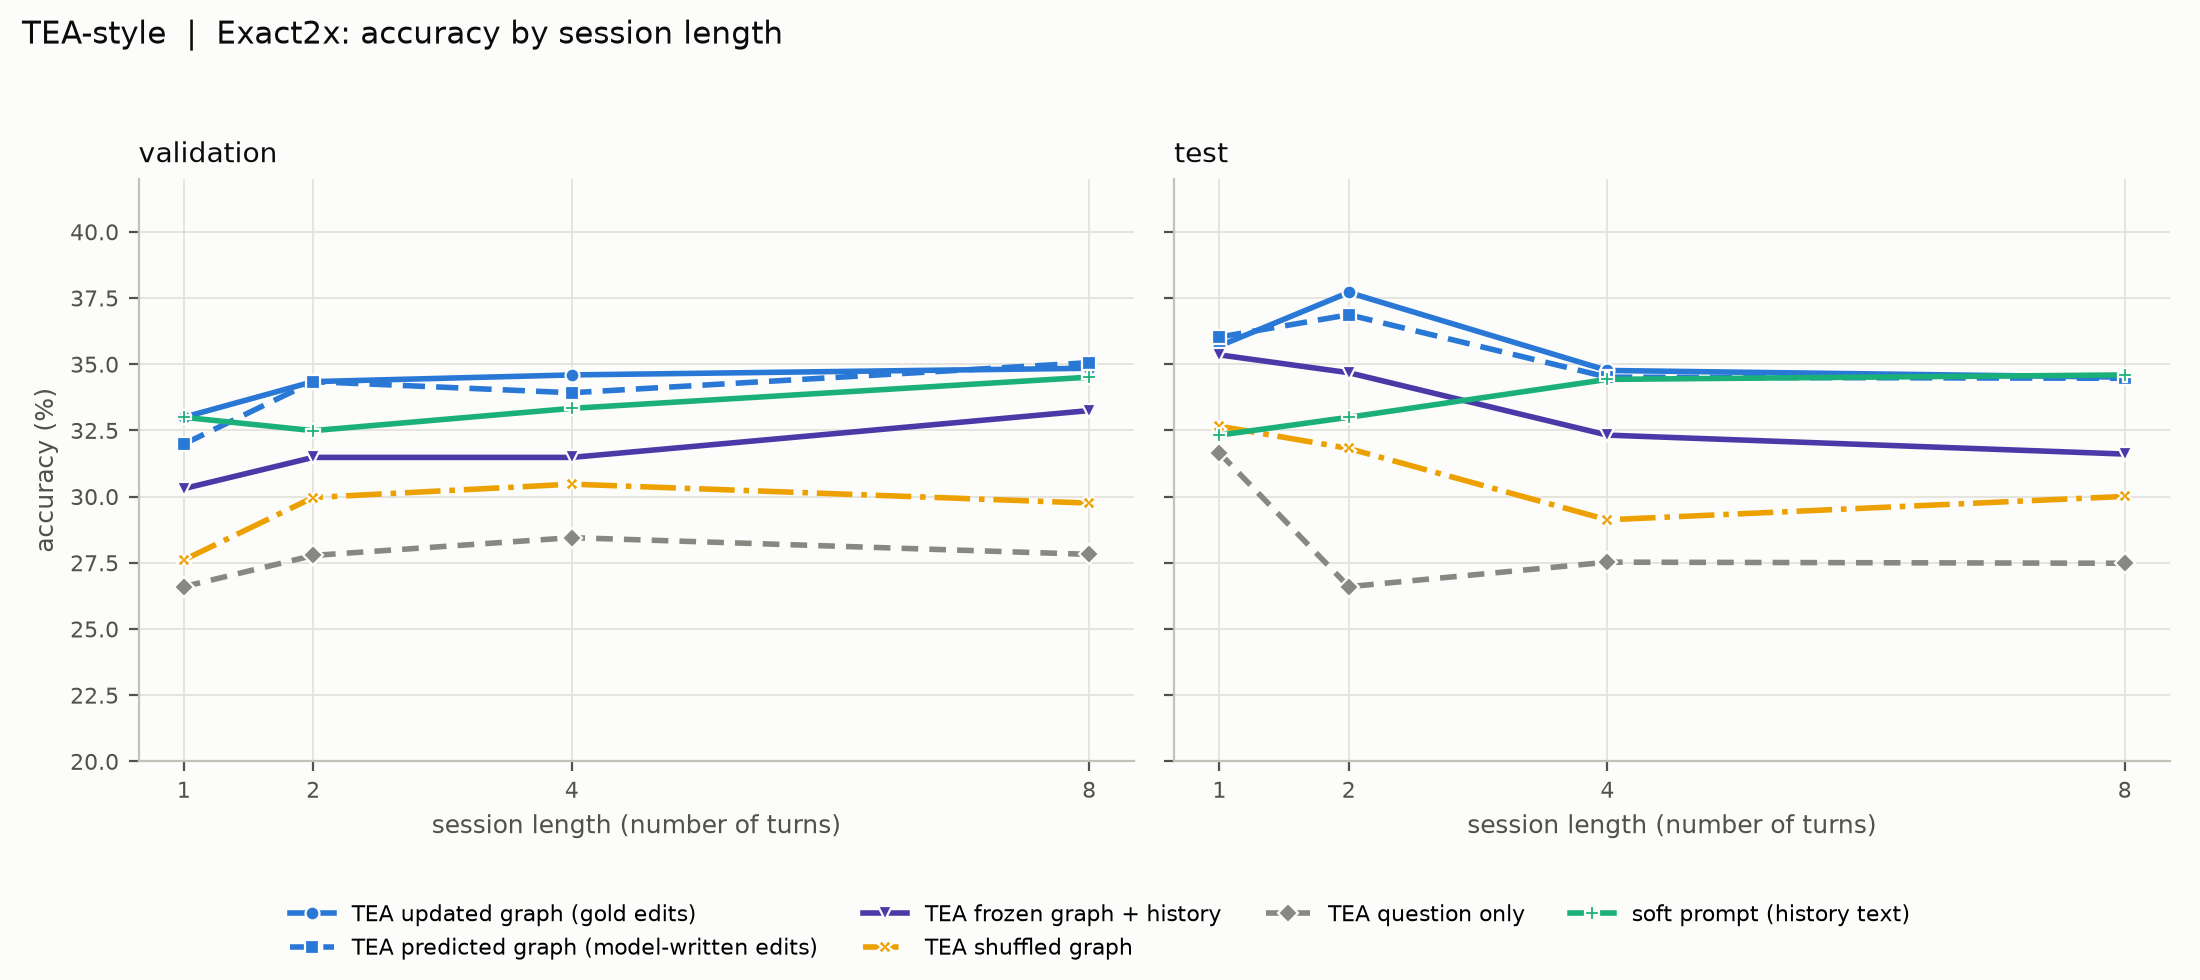
\includegraphics[width=\linewidth]{figures/tea_fig1_accuracy_by_session_length.png}\\[2pt]
  {\small (a) TEA-style, by session length}
\end{minipage}\hfill
\begin{minipage}[t]{0.48\textwidth}
  \centering
  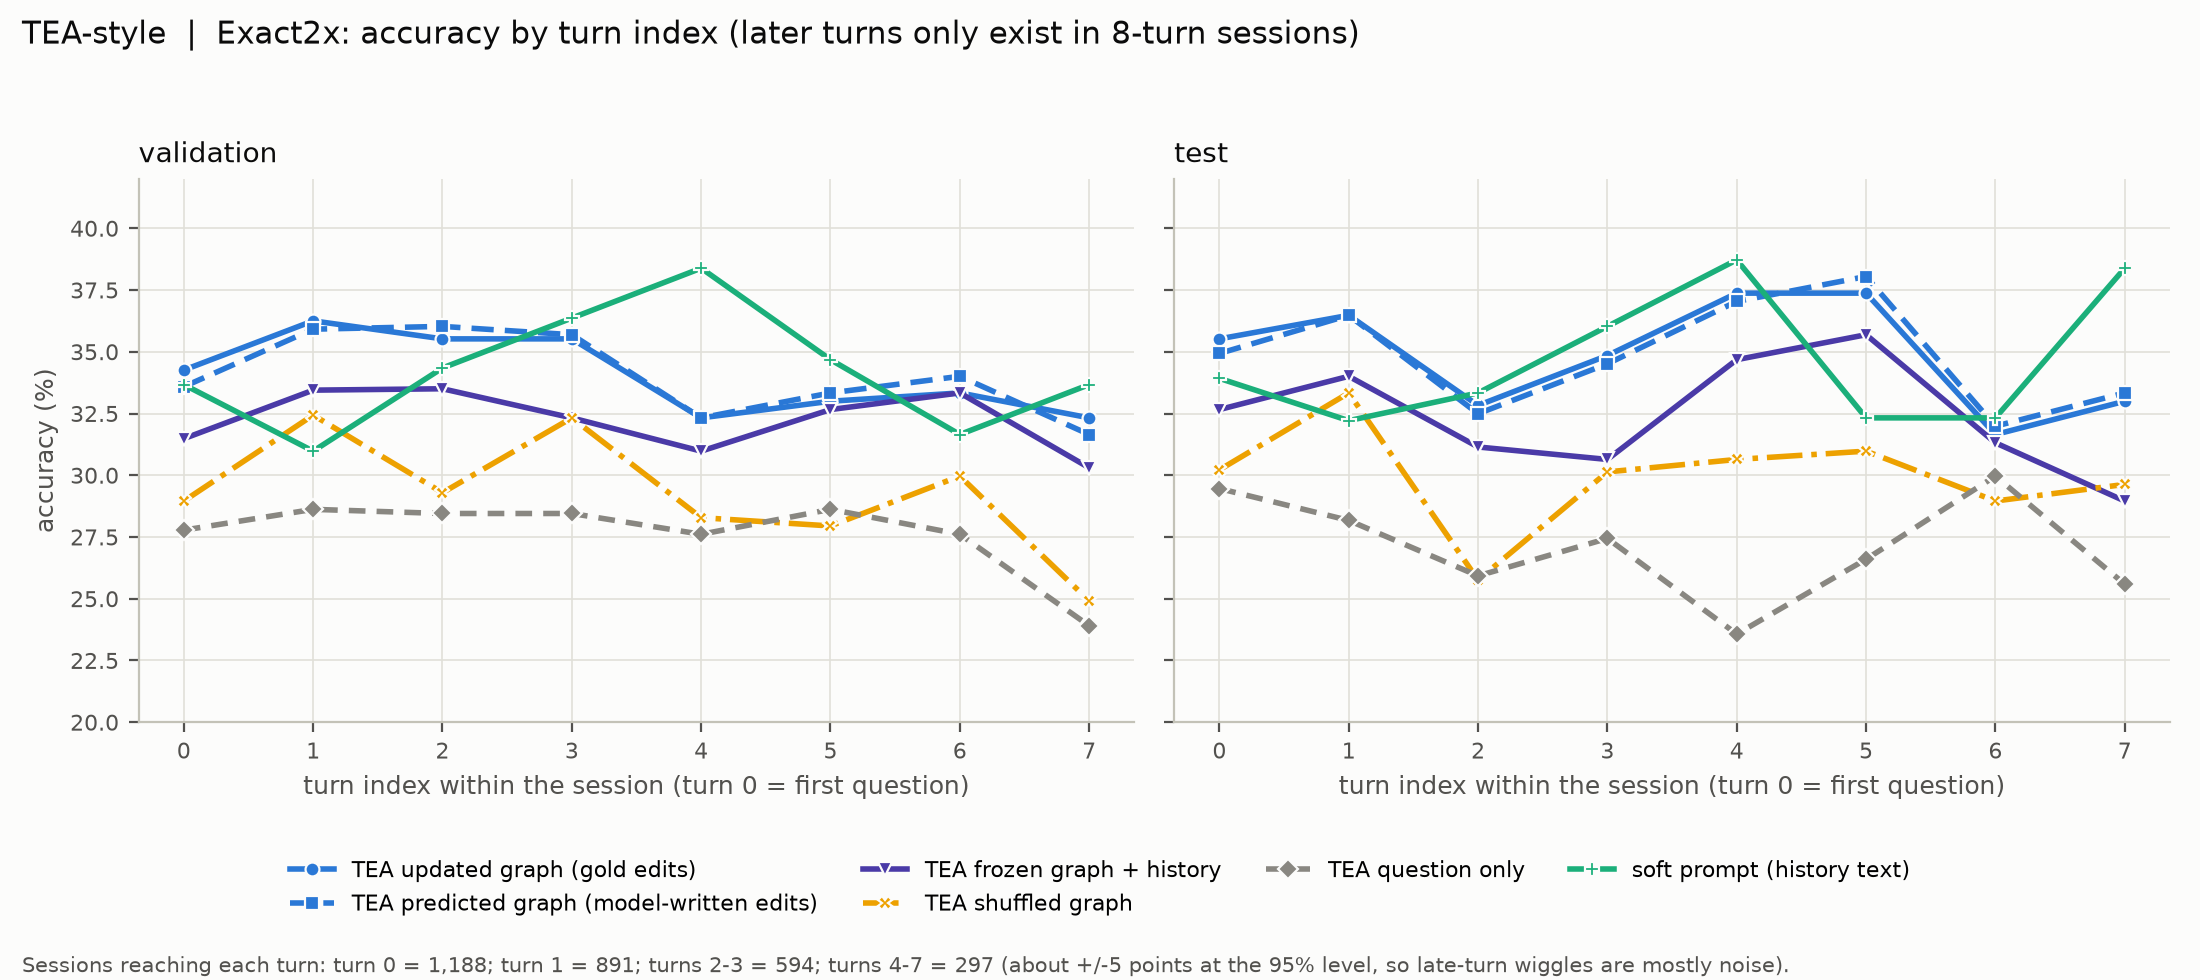
\includegraphics[width=\linewidth]{figures/tea_fig2_accuracy_by_turn_index.png}\\[2pt]
  {\small (b) TEA-style, by turn index}
\end{minipage}\\[8pt]
\begin{minipage}[t]{0.48\textwidth}
  \centering
  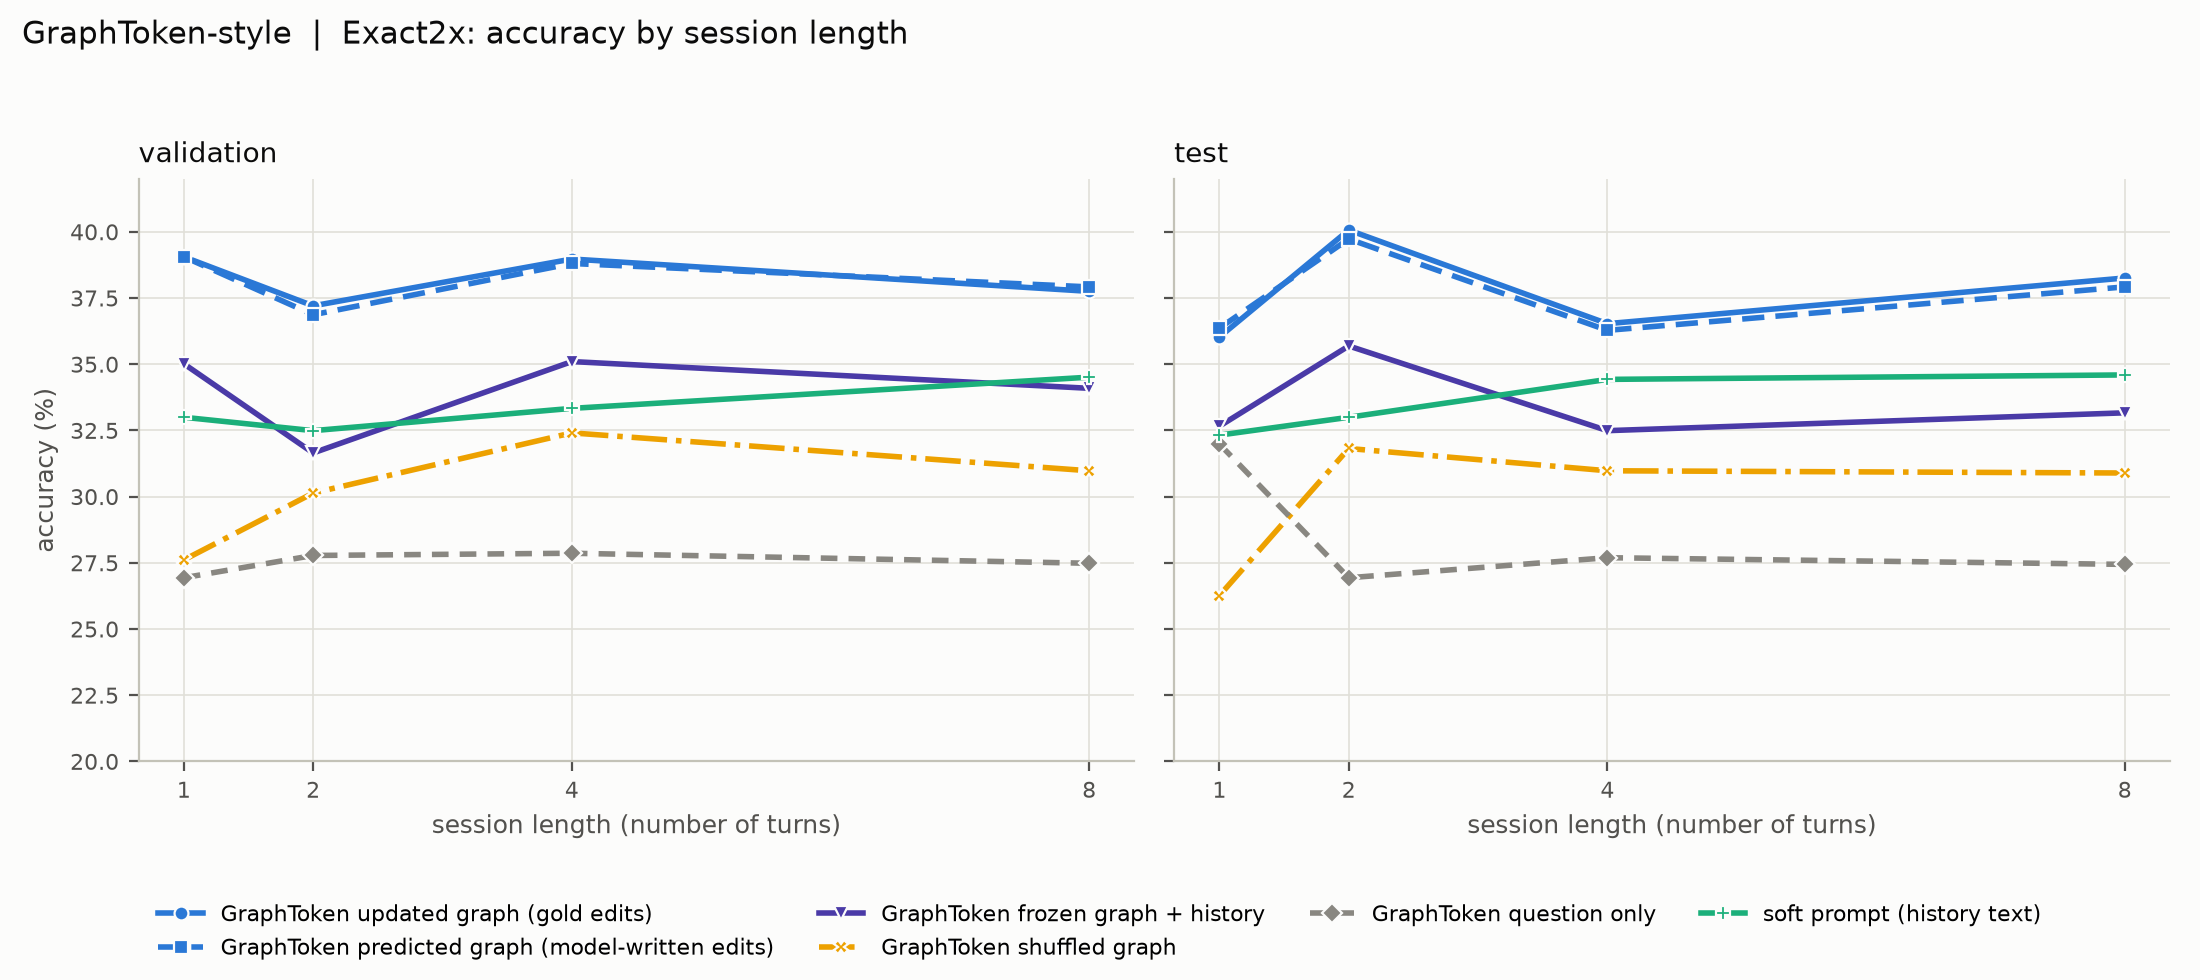
\includegraphics[width=\linewidth]{figures/graphtoken_fig1_accuracy_by_session_length.png}\\[2pt]
  {\small (c) GraphToken-style, by session length}
\end{minipage}\hfill
\begin{minipage}[t]{0.48\textwidth}
  \centering
  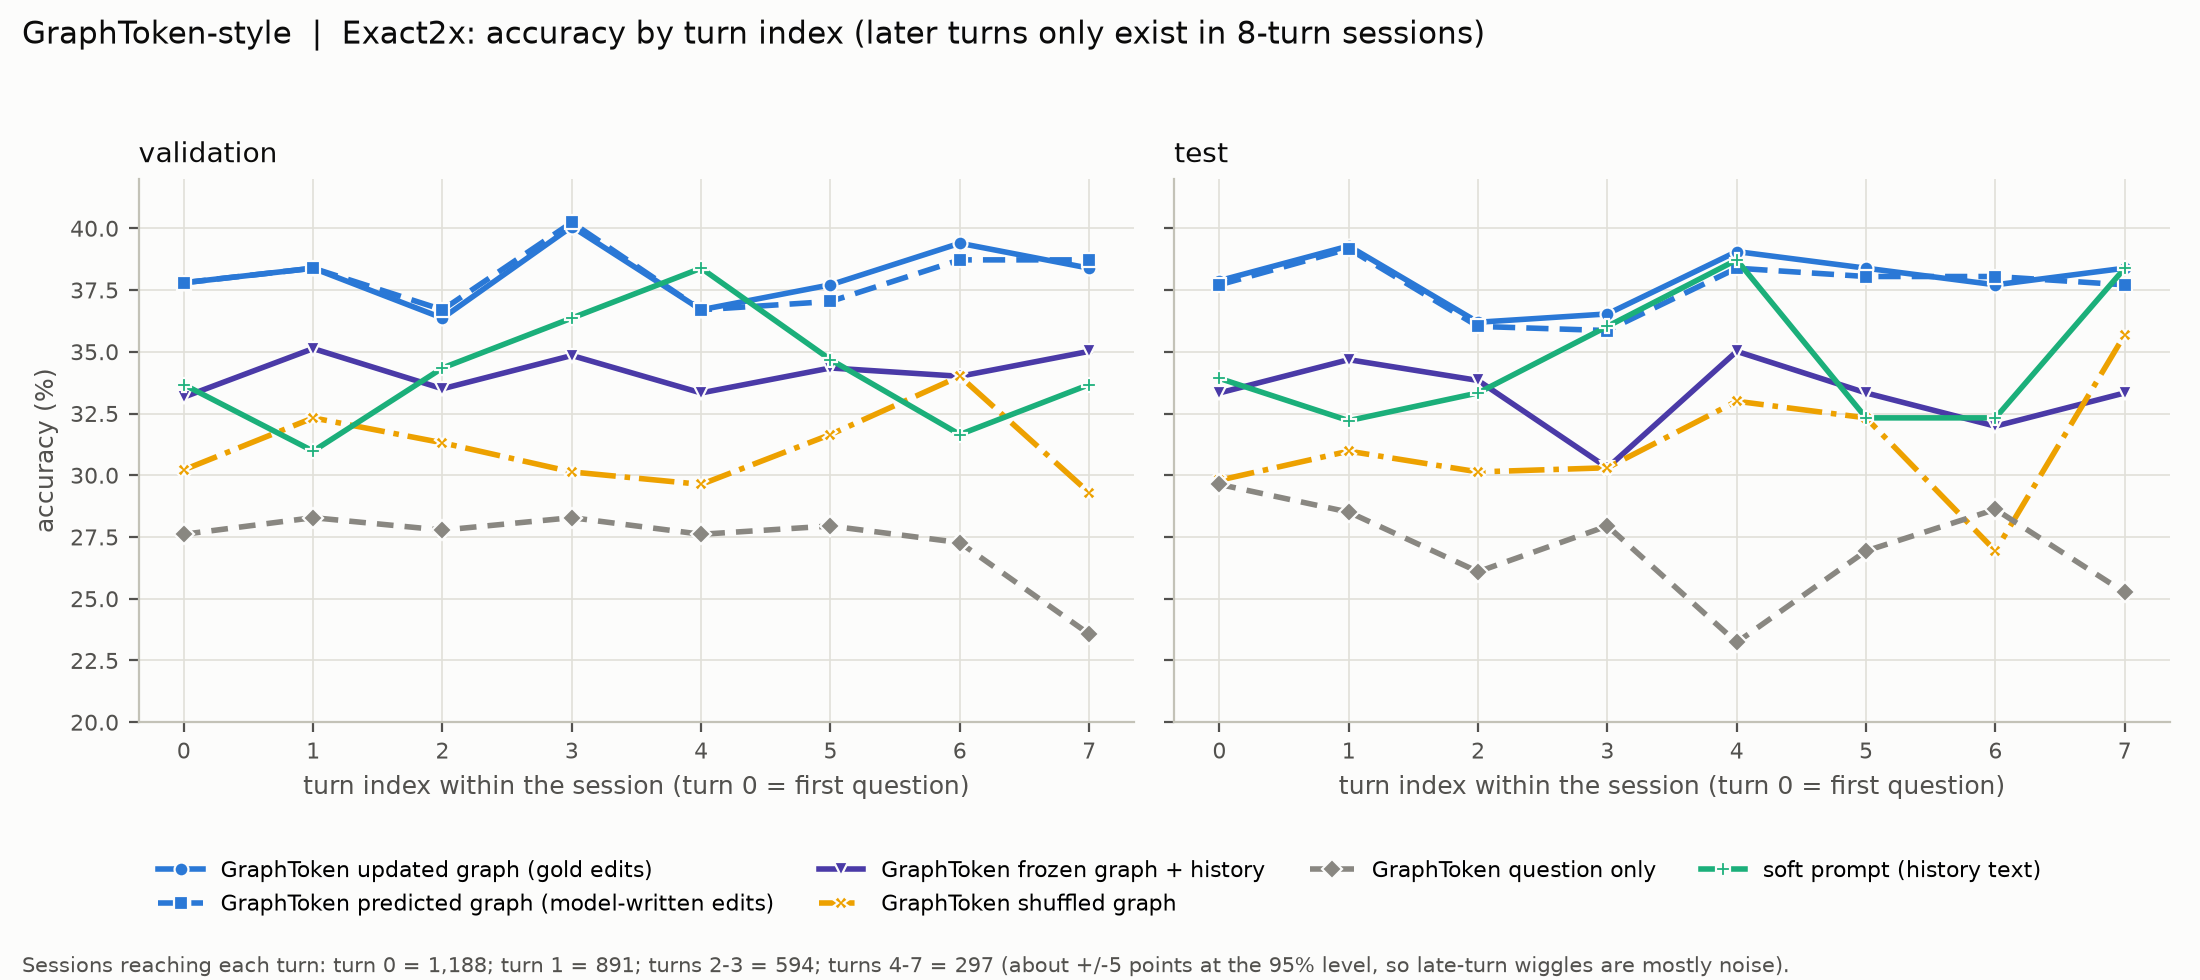
\includegraphics[width=\linewidth]{figures/graphtoken_fig2_accuracy_by_turn_index.png}\\[2pt]
  {\small (d) GraphToken-style, by turn index}
\end{minipage}
\caption{Multi-turn accuracy by session length (left column) and by turn index (right column), for the TEA-style model (top row) and the GraphToken-style model (bottom row). On test, TEA-style with stale graph tokens plus history falls from 35.4\% to 31.6\% between 1- and 8-turn sessions, while re-encoded tokens (gold and model-written edits) stay near 35\%. GraphToken-style stale tokens do not show a steady decline. The soft prompt (green) reads the revision history as text. In the right column, later turns only occur in 8-turn sessions (297 sessions), so differences between individual late turns are within noise.}
\label{fig:multiturn}
\end{figure*}

\begin{table}[t]
\centering
\small
\resizebox{\linewidth}{!}{%
\begin{tabular}{@{}lcccc@{}}
\toprule
\textbf{Condition} & \textbf{1} & \textbf{2} & \textbf{4} & \textbf{8} \\
\midrule
oracle\_updated\_graph & 35.7 & 37.7 & 34.8 & 34.5 \\
predicted\_updated\_graph & 36.0 & 36.9 & 34.5 & 34.5 \\
frozen\_graph\_history / cached\_no\_reencode & 35.4 & 34.7 & 32.3 & 31.6 \\
graph\_once\_then\_text & 34.7 & 28.6 & 29.2 & 29.8 \\
shuffled\_graph & 32.7 & 31.8 & 29.1 & 30.0 \\
question\_only & 31.6 & 26.6 & 27.5 & 27.5 \\
soft\_prompt & 32.3 & 33.0 & 34.4 & 34.6 \\
\bottomrule
\end{tabular}}
\caption{Test accuracy (\%) by session length (TEA-style, soft prompt). The predicted row is from a separate run whose oracle row is 36.4/37.4/34.7/34.5.}
\label{tab:length}
\end{table}

Figure~\ref{fig:multiturn} and Table~\ref{tab:length} address RQ2.
On the test split, TEA-style re-encoded tokens hold their accuracy across session lengths while stale tokens lose accuracy as edits accumulate.
The GraphToken-style panels (bottom row) show the same ordering of conditions.
Model-written edits track oracle edits mostly at every length for both models.
\texttt{frozen\_graph\_history} drops 3.8 points from 1- to 8-turn sessions.
\texttt{graph\_once\_then\_text}, which sees the graph only at the first turn, drops 6.1 points after the first edit and stays there.
The length trend does not replicate on validation, where \texttt{frozen\_graph\_history} rises from 30.3\% to 33.2\%; re-encoding is still ahead of it at every length, by 1.6 to 3.1 points.

The soft prompt does not degrade and rises slightly with session length (32.3\% to 34.6\%).
It receives the accumulated revision text, so changes such as ``X is closed now'' can answer later reachability questions directly. We also hypothesize that the reason for this is it is encoding the dataset distribution rather than the graph and since each turn questions are made using the same static QA benchmark, across turns, the soft prompt holds its accuracy. 

\begin{table}[t]
\centering
\small
\resizebox{\linewidth}{!}{%
\begin{tabular}{@{}lcccc@{}}
\toprule
 & \multicolumn{2}{c}{\textbf{Changed}} & \multicolumn{2}{c}{\textbf{Unchanged}} \\
\textbf{Condition} & Val & Test & Val & Test \\
\midrule
oracle\_updated\_graph & 34.4 & 34.6 & 34.7 & 35.4 \\
predicted\_updated\_graph & 34.5 & 34.2 & 34.4 & 35.4 \\
frozen\_graph\_history / cached\_no\_reencode & 29.3 & 29.7 & 34.4 & 34.4 \\
question\_only & 26.6 & 25.5 & 28.7 & 29.2 \\
soft\_prompt & 33.8 & 33.0 & 33.8 & 35.0 \\
\bottomrule
\end{tabular}}
\caption{Accuracy (\%) on answer-changing vs.\ unchanged turns. Test: 1{,}811 changed and 2{,}644 unchanged turns; validation: 1{,}790 and 2{,}665.}
\label{tab:changing}
\end{table}

Table~\ref{tab:changing} and Figure~\ref{fig:edit} (Appendix~\ref{app:edit}) split turns by whether the edit changed the answer.
On unchanged turns, TEA-style stale and re-encoded tokens are within one point of each other on both splits, as expected.
On changed turns, TEA-style re-encoding beats stale tokens by 4.9 points on test (34.6 vs.\ 29.7) and 5.1 on validation (34.4 vs.\ 29.3).
TEA-style re-encoded accuracy is the same on changed and unchanged turns, which is what a model reading the current graph should show.
GraphToken-style shows a larger staleness effect on changed turns (Figure~\ref{fig:edit}, bottom): re-encoding scores 33.2\% with gold edits and 32.6\% with model-written edits against 24.4\% for stale tokens plus history, a gap of 8.8 and 8.2 points on test.
Its accuracy is higher on unchanged turns (41.1\% re-encoded, 39.4\% stale), so unlike TEA-style it does not score the same on changed and unchanged turns.

\subsection{Density and task breakdown}
\label{sec:breakdown}

\begin{table}[t]
\centering
\small
\begin{tabular}{@{}lccc@{}}
\toprule
 & \textbf{Sparse} & \textbf{Medium} & \textbf{Dense} \\
\midrule
oracle\_updated\_graph & 34.0 & 35.9 & 35.4 \\
predicted\_updated\_graph & 33.9 & 35.5 & 35.4 \\
shuffled\_graph & 29.9 & 31.2 & 29.5 \\
soft\_prompt & 33.3 & 34.7 & 34.5 \\
\bottomrule
\end{tabular}
\caption{Test accuracy (\%) by graph density.}
\label{tab:density}
\end{table}

\begin{table}[t]
\centering
\small
\resizebox{\linewidth}{!}{%
\begin{tabular}{@{}lcccccc@{}}
\toprule
\textbf{Task} & \textbf{Oracle} & \textbf{Pred.} & \textbf{Shuffled} & \textbf{Q only} & \textbf{Soft} & \textbf{Maj.} \\
\midrule
reachability & 60.6 & 59.2 & 52.1 & 50.3 & 61.2 & 50.3 \\
constrained\_reachability & 55.4 & 55.6 & 48.3 & 49.9 & 51.3 & 50.1 \\
cycle\_membership & 53.5 & 53.9 & 51.1 & 49.7 & 57.2 & 50.3 \\
edge\_exists & 50.1 & 49.7 & 49.9 & 48.9 & 53.9 & 50.1 \\
most\_common\_attr.\ within hops & 33.1 & 32.9 & 19.4 & 0.0 & 26.5 & 6.3 \\
shortest\_path & 18.6 & 18.6 & 16.6 & 14.3 & 18.6 & 17.6 \\
node\_degree & 16.8 & 16.6 & 11.7 & 12.7 & 11.7 & 12.9 \\
filtered\_neighbor\_count & 14.9 & 14.7 & 12.9 & 16.0 & 16.8 & 17.2 \\
within\_hops\_count & 12.7 & 12.9 & 9.7 & 7.1 & 10.5 & 9.9 \\
\bottomrule
\end{tabular}%
}
\caption{Multi-turn test accuracy (\%) by task for the TEA-style conditions and the soft prompt ($n{=}495$ per task).}
\label{tab:pertask}
\label{tab:task-breakdown}
\end{table}

Tables~\ref{tab:density} and~\ref{tab:pertask} break the test results down.
Accuracy varies by less than 2 points across densities, and re-encoding is ahead of the shuffled graph at every density by 4.1 to 5.9 points.
By task, the graph helps most on most-common attribute within hops (33.1\% vs.\ 19.4\% shuffled and 0.0\% for \texttt{question\_only}) and on the reachability family (55--61\% vs.\ about 50\%).
The soft prompt matches or beats re-encoding on reachability, cycle membership, and edge existence, which are the yes/no tasks where revision text such as ``X is closed'' is most directly informative.
All models are near the majority rate on the count tasks.

\subsection{Write path}
\label{sec:write}

The \texttt{predicted\_updated\_graph} condition applies the model's own edit programs and re-encodes the result, and it answers RQ1.
The frozen LLM reproduces the gold edit exactly on 95.2\% of test turns, and the resulting graph state is exactly right on 88.6\% test turns.
NOOP turns are always correct, and the weakest operation is \texttt{ADD EDGE} at 89.9\%; the other edit kinds are between 91.7\% and 93.9\%.
With these edits, TEA-style scores 34.9\% against 35.0\% for the gold edits in the same run, and GraphToken-style scores 37.6\% against 37.9\% (Table~\ref{tab:conditions}).
The predicted and oracle rows also agree within 1.4 points by session length, change status, density, and task (Tables~\ref{tab:length}--\ref{tab:pertask}), so edit errors are cheap on this benchmark.

\section{Inferences}
\label{sec:discussion}

\paragraph{Graph tokens encode the specific graph.}
For static QA, both graph models perform better than the soft prompt (RQ3), and in multi-turn sessions the correct graph beats a shuffled one by 4.9 points on test and 4.8 on validation, at every density.
The gap is largest on the task that depends more on node attributes such as the most-common attribute within hops is 33.1\% with the correct graph, 19.4\% with a shuffled one, and 0.0\% without graph tokens.
A model that ignored the tokens would score the same under all three, so the tokens carry session-specific information.

\paragraph{Staleness hurts exactly where an edit matters.}
On turns where the edit changed the answer, re-encoded tokens beat stale ones by about 5 points on both splits and on unchanged turns the two are within one point.
Re-encoded accuracy is also nearly the same on changed and unchanged turns (34.6 vs.\ 35.4 on test), while stale accuracy drops by about 5 points on changed turns.
This pattern is what a model that reads the current graph should show, and it supports RQ2 more directly than the session-length trend, which appears on test but not on validation.

\paragraph{The gain comes from re-encoding, not from text history.}
Adding the revision text to stale tokens does not help the graph model as the \texttt{frozen\_graph\_history} and \texttt{structure\_only} are within 0.4 points on both splits (32.5 vs.\ 32.3 on test).
History text alone (\texttt{token\_matched\_history}) is 1.3 points above \texttt{question\_only} on test.
So the 2.6-point test gap between re-encoded and stale tokens is not recovered by putting the edits into the prompt.

\paragraph{Graph tokens and revision text help different tasks.}
Soft prompt with the revision history matches and sometimes beat re-encoding on the yes/no tasks where a revision such as ``X is closed'' is directly informative on tasks like reachability (61.2 vs.\ 60.6), cycle membership (57.2 vs.\ 53.5), and edge existence (53.9 vs.\ 50.1).
Re-encoding is ahead where the answer depends on graph structure or attributes that the revisions do not state such as most-common attribute within hops (33.1 vs.\ 26.5), constrained reachability (55.4 vs.\ 51.3), node degree (16.8 vs.\ 11.7) and within-hops count (12.7 vs.\ 10.5).

\paragraph{Limits of the evidence.}
Overall, re-encoding is 0.9 points above the soft prompt, one seed cannot tell whether that margin is real, and the soft prompt sees the history, so we do not claim that graph tokens beat a text channel.
Absolute accuracy is about 35\%, and count tasks stay below 20\%, so the read path is the main bottleneck rather than state tracking.
Finally, predicted edits lose almost nothing here (0.1 to 0.3 points), but the revisions are templated, so this likely overstates the write path on free-form dialogue.

\section{Future Timeline}
\label{sec:timeline}

\begin{table}[t]
\centering
\small
\begin{tabular}{@{}lp{0.62\linewidth}@{}}
\toprule
\textbf{Status} & \textbf{Item} \\
\midrule
Done & Edit language, executor, few-shot edit prompt \\
Done & BERT/GraphSAGE read path; TEA-style, GraphToken-style and soft-prompt training \\
Done & Multi-turn grid and paired conditions for TEA-style, GraphToken-style and soft prompt \\
Done & Predicted-edit evaluation (TEA-style and GraphToken-style) \\
Done & Joint GraphToken training \\
Open & Serialized graph input \\
Open & Contradiction probe (Logical contradiction) \\
Open & Ablations on GLM architecture \\
Open & Multiple seeds for final experiments and results \\
\bottomrule
\end{tabular}
\caption{Status relative to the proposal.}
\label{tab:status}
\end{table}

\begin{table}[t]
\centering
\small
\begin{tabular}{@{}lp{0.62\linewidth}@{}}
\toprule
\textbf{Window} & \textbf{Work} \\
\midrule
Oct 1--4 & Serialized graph input and then evaluation on benchmark \\
Oct 5--10 & 3--5 seeds of TEA, GraphToken and soft prompt. \\
Oct 11--21 & Ablations: always-mean pooling, no contrastive pretraining, soft prompt without history text. \\
Oct 22--31 & Contradiction probe; final report. \\
\bottomrule
\end{tabular}
\caption{October schedule.}
\label{tab:october}
\end{table}

Tables~\ref{tab:status} and~\ref{tab:october} give the plan. The main points are expanding the benchmark to include a logical contradiction application where the multi-turns evolve into a logical and sematic contraction such as; A is father of B, B is father of C, C is father of A; is flagged by the GLM as erroneous. We also hope to complete multiple seed runs for all of our experiments and report CI and other relevant metrics. 

\section*{Limitations}

We evaluate an LLM with just one seed.
Revisions follow a template, so edit accuracy will likely overstate performance on free-form dialogue.
Edit prediction uses one few-shot prompt, and 11\% of test graph states are wrong, so the small accuracy cost may not hold for harder revisions.

\bibliography{custom}

\clearpage
\appendix

\section{Accuracy on Answer-Changing Turns}
\label{app:edit}

\begin{figure}[h]
\centering
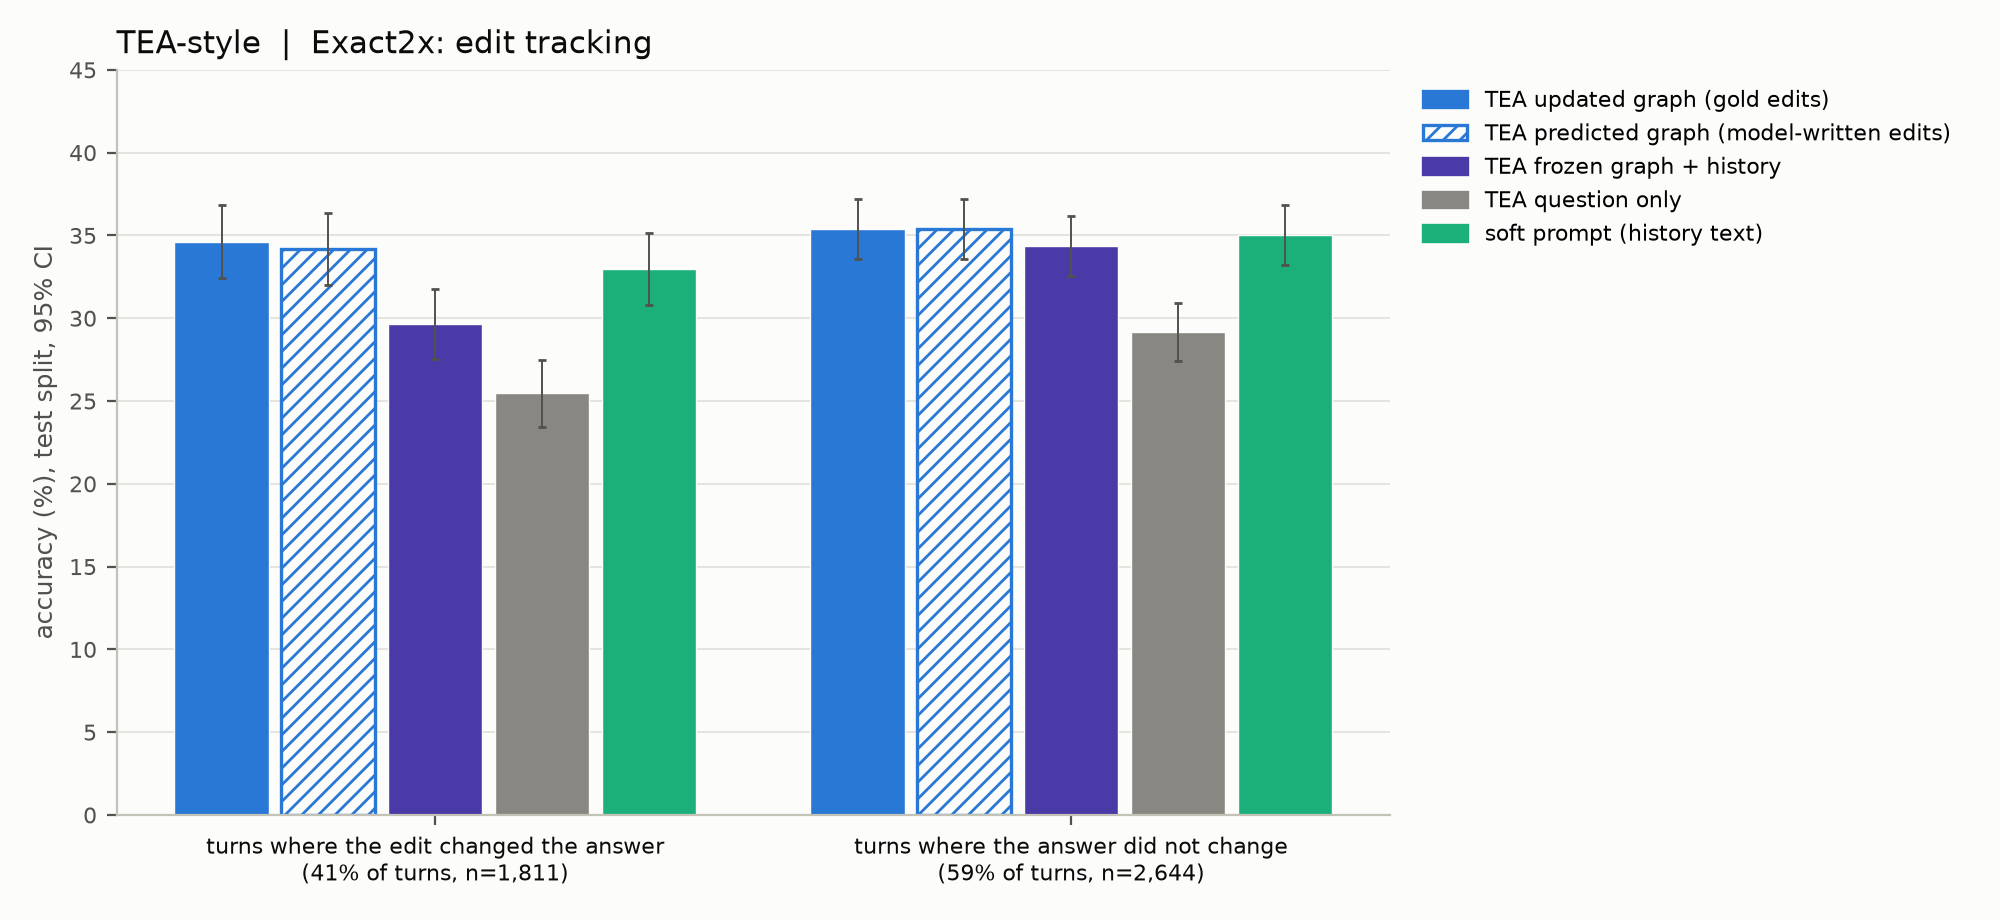
\includegraphics[width=\linewidth]{figures/tea_fig3_edit_tracking.png}\\[4pt]
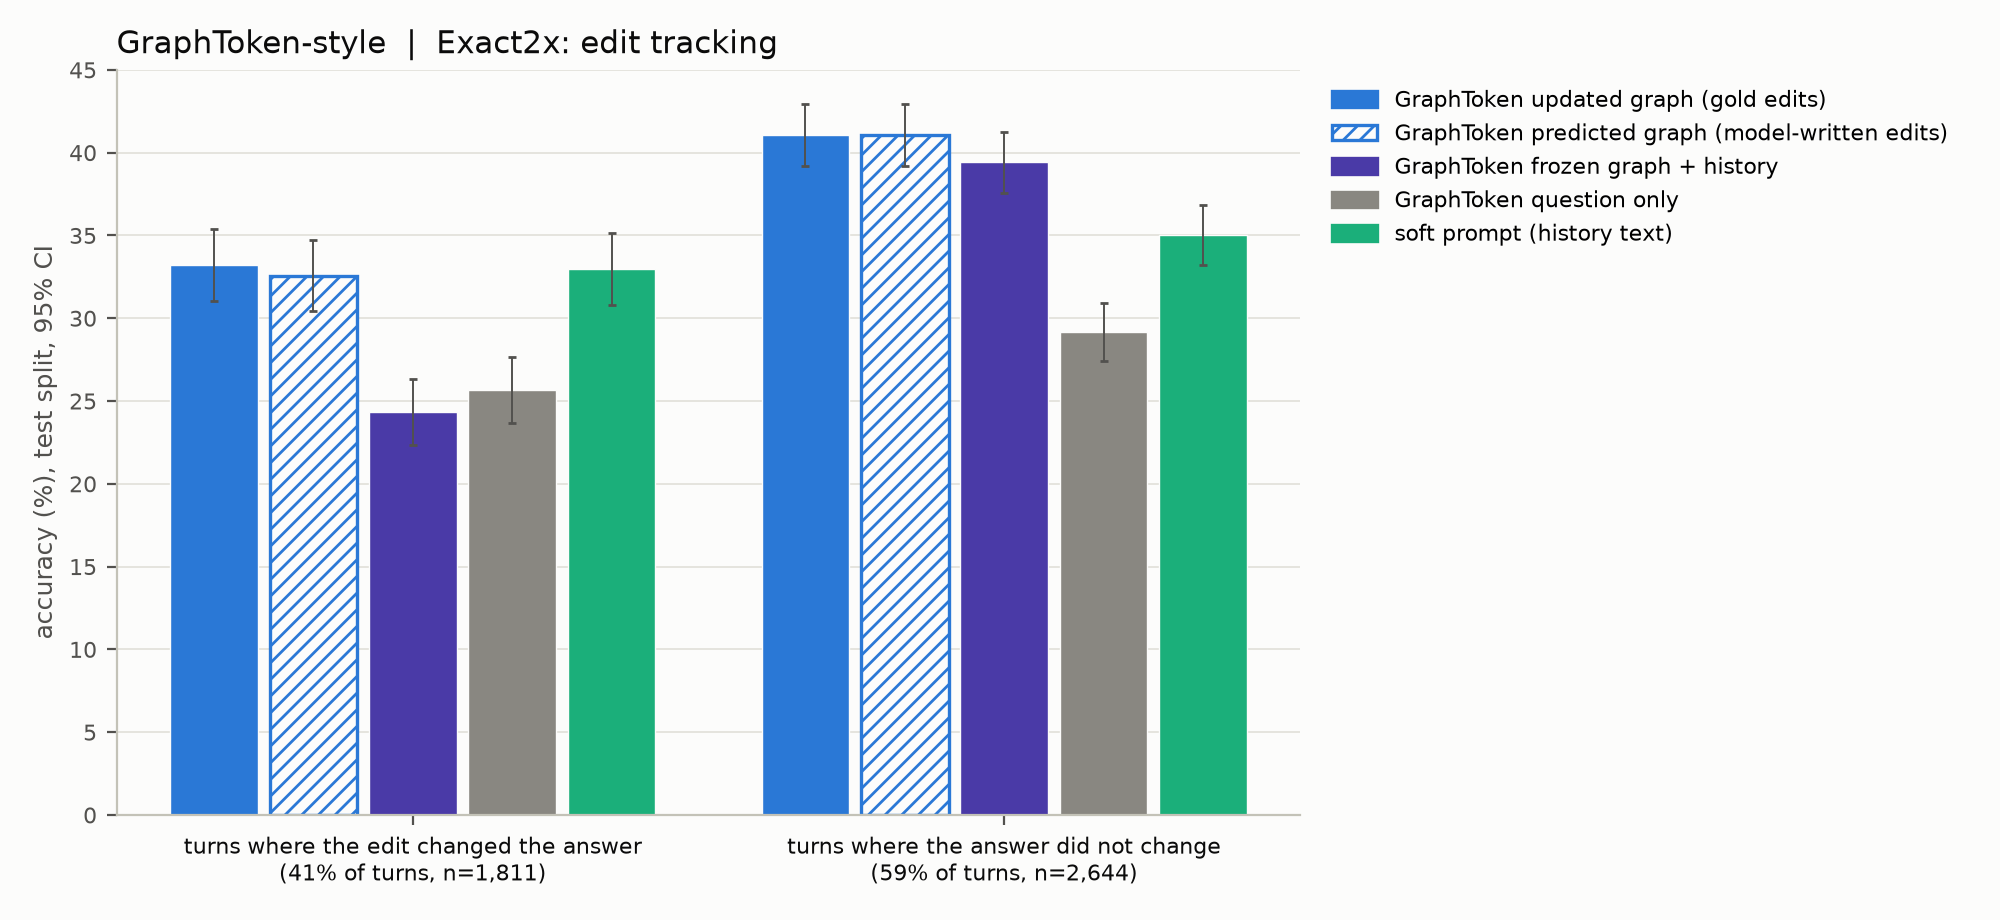
\includegraphics[width=\linewidth]{figures/graphtoken_fig3_edit_tracking.png}
\caption{Test accuracy on turns where the edit changed the answer (41\%) and where it did not (59\%), for the TEA-style model (top) and the GraphToken-style model (bottom). Error bars are binomial 95\% intervals over turns from one seed; they do not reflect seed variance.}
\label{fig:edit}
\end{figure}

\section{TEA-style and GraphToken-style Multi-Turn Results}
\label{app:combined}

\begin{figure*}[p]
\centering
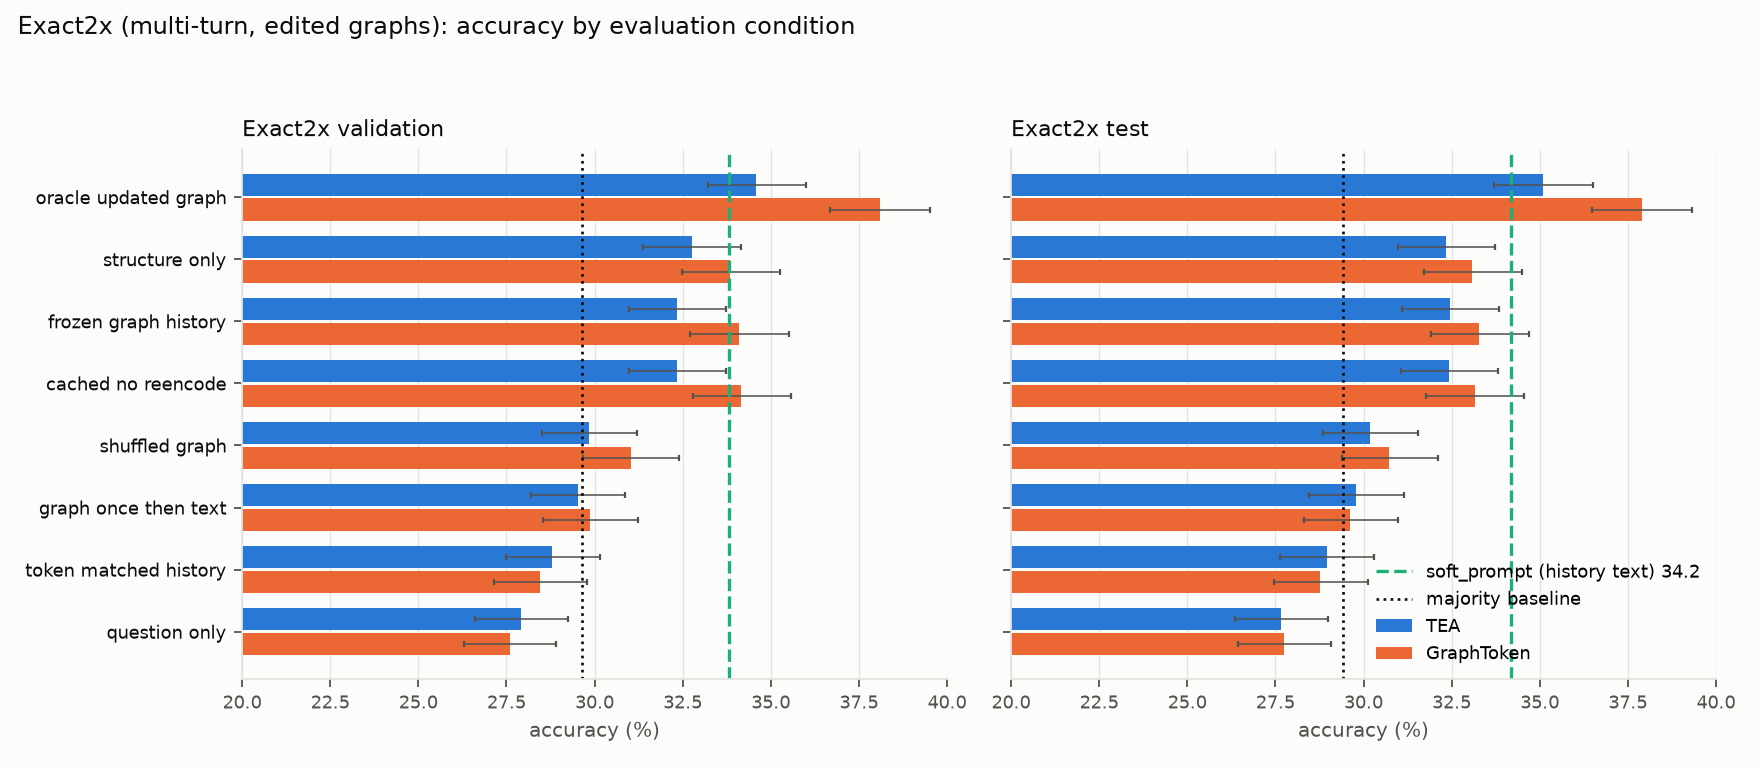
\includegraphics[width=0.95\textwidth,height=0.29\textheight,keepaspectratio]{figures/v3_combined_conditions.png}\\[4pt]
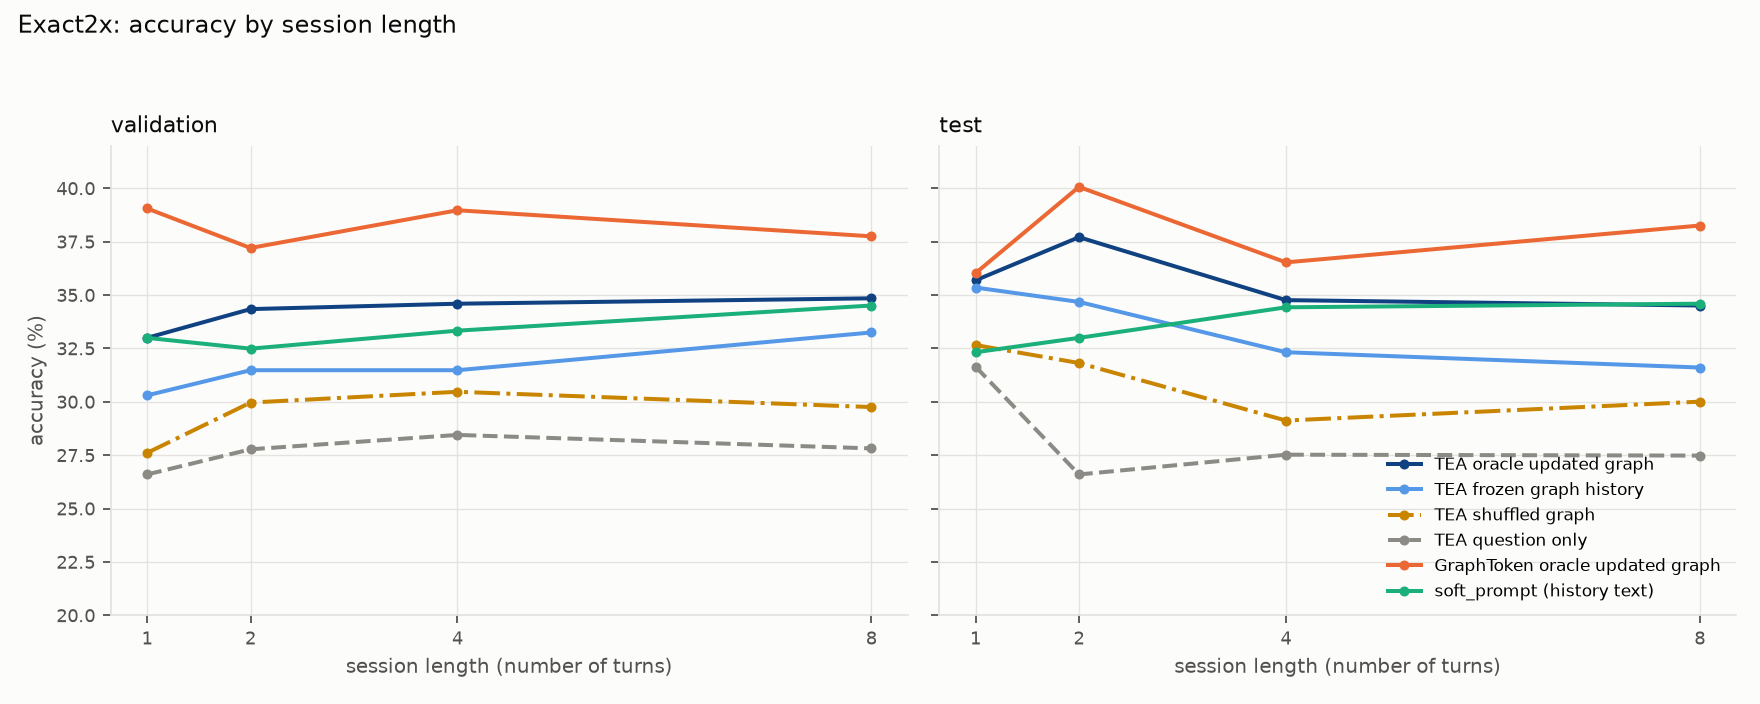
\includegraphics[width=0.95\textwidth,height=0.29\textheight,keepaspectratio]{figures/v3_combined_by_session_length.png}\\[4pt]
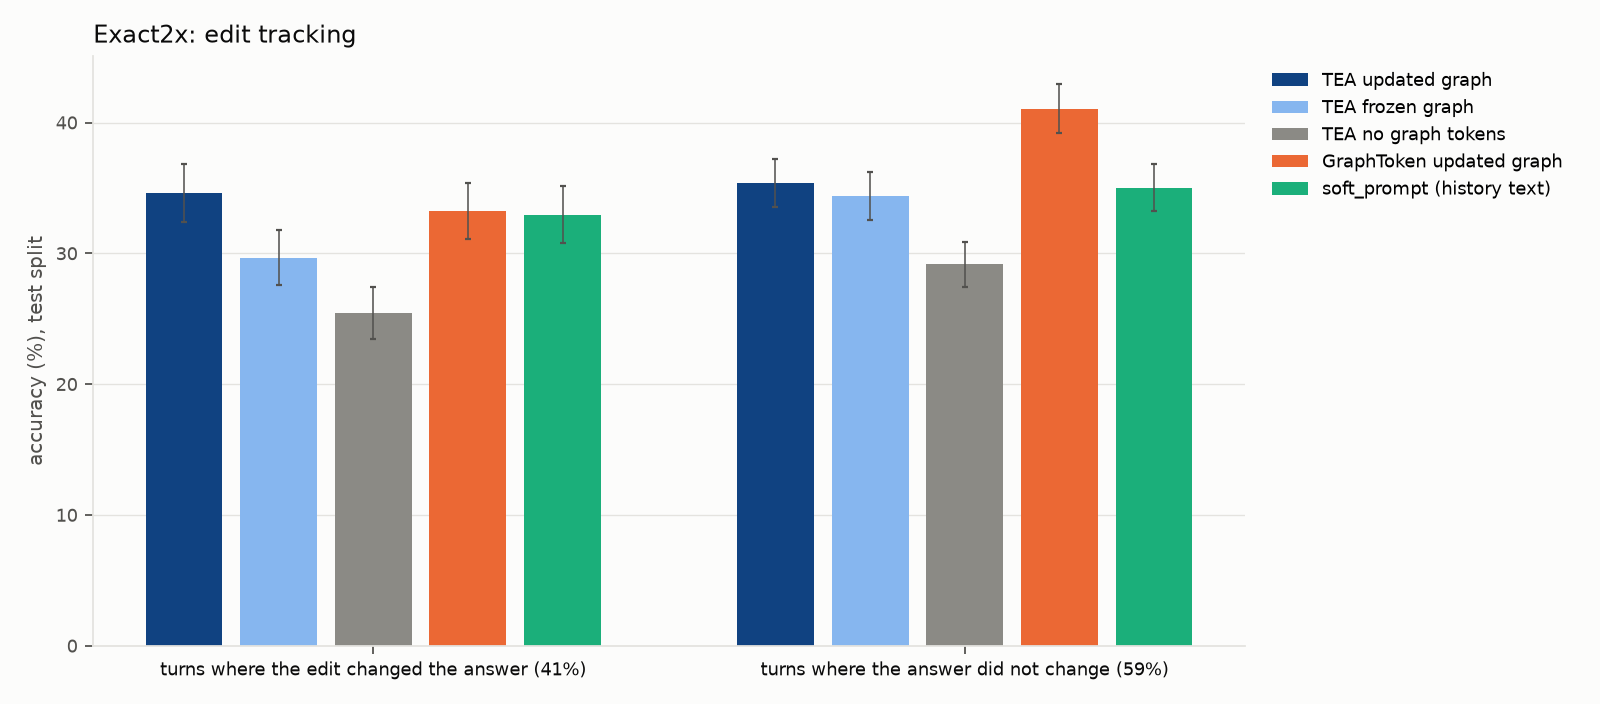
\includegraphics[width=0.95\textwidth,height=0.29\textheight,keepaspectratio]{figures/v3_combined_edit_tracking.png}
\caption{Multi-turn results for the TEA-style model (blue) and the GraphToken-style model (orange), with the soft prompt (green) for reference. Top: accuracy under each condition on validation and test. Middle: accuracy by session length. Bottom: test accuracy on turns where the edit changed the answer and where it did not. On test, re-encoding the gold graph gives 37.9\% for GraphToken-style and 35.1\% for TEA-style; the shuffled graph gives 30.7\% and 30.2\%. Error bars are binomial 95\% intervals over turns from one seed.}
\label{fig:combined}
\end{figure*}

\section{All Conditions for TEA-style and GraphToken-style}
\label{app:allconds}

Figures~\ref{fig:allA1}--\ref{fig:allA3} repeat the main-text plots with every condition of Table~\ref{tab:conditions-def}, for the TEA-style model (top of each figure) and the GraphToken-style model (bottom).
In the upper panels of each plot the graph-token conditions are shown, and in the lower panels the text-only conditions and the two reference points (stale answer and per-task majority).
The stale-answer reference is 0\% on answer-changing turns and 100\% on unchanged turns by definition.



\section{Task Families}
\label{app:task-families}

Static QA covers eleven task families; the multi-turn grid uses the first nine. Every answer is
computed by a symbolic solver on the current graph, and yes/no tasks are balanced 50/50. In the
definitions below, A and B are station names.
\begin{itemize}
  \item \textbf{Edge existence}: is there a direct edge between A and B? Negatives are split
  evenly between pairs that share a neighbour and pairs that do not.
  \item \textbf{Reachability}: can B be reached from A using open stations only?
  \item \textbf{Constrained reachability}: can B be reached from A without passing through a
  station of a given class (no disabled access, no rail, or dirty)?
  \item \textbf{Cycle membership}: is A part of any cycle?
  \item \textbf{Node degree}: how many stations are directly connected to A?
  \item \textbf{Filtered neighbour count}: how many direct neighbours of A have a given
  attribute value (accessibility, rail, line, architecture or cleanliness)?
  \item \textbf{Shortest path}: how many stations, including both endpoints, lie on the shortest
  open path from A to B (or \texttt{unreachable})?
  \item \textbf{Within-hops count}: how many other stations within two hops of A have a given
  attribute value?
  \item \textbf{Most common attribute within hops}: what is the most common value of an attribute
  (line, architecture, cleanliness, music or size) among the stations within two hops of A,
  including A itself? Only queries with a unique mode are kept.
  \item \textbf{Attribute lookup}: what is the value of one of A's attributes (architecture,
  cleanliness, music, size or line)? The answer is an open categorical value.
  \item \textbf{Attribute check}: does A have a given attribute value? This asks the same kind of
  fact as attribute lookup, as a yes/no question.
\end{itemize}
The last two are CLEGR's Facts tasks. For them, and for the most-common-attribute task, the
queried attribute is withheld from W(f\textsubscript{i}), so the answer cannot be read from the
question text and has to come from the graph tokens. The Facts tasks are static only: revisions
toggle station status or add and remove edges, so they never change a node attribute, and a
Facts question could never become an answer-changing turn.

\paragraph{Static accuracy by task family.} Figures~\ref{fig:static-tasks-tea}
and~\ref{fig:static-tasks-gt} break the static results of Table~4 down by task family for each
graph model, against the soft prompt, the question-only prior (the best rule using only the
question fields) and the per-task majority answer. On the nine multi-turn tasks the pattern
matches Table~\ref{tab:task-breakdown}: the graph tokens help on reachability (test: TEA-style
57.8\%, GraphToken-style 68.9\%, soft prompt 50.0\%), constrained reachability (53.8\%, 61.1\%,
48.0\%) and the most common attribute within hops (32.3\%, 50.0\%, 28.0\%), and every model stays
near the prior on the count tasks (node degree, filtered neighbour count, within-hops count,
shortest path), all below 20\%.

The two Facts tasks behave differently from each other. On \textbf{attribute lookup} both graph
models are well above the 27.3\% question-only prior on test, TEA-style at 43.2\% and
GraphToken-style at 54.5\% (validation: 48.5\% and 56.6\%), while the soft prompt stays at the
prior (27.3\%; validation 29.8\%). Because the queried attribute is withheld from the question,
this gain can only come from the graph tokens, and it is the clearest sign that the tokens carry
the named station's own attributes. On \textbf{attribute check}, which asks about the same kind
of fact as a yes/no question, every model is at chance: 48.2\% (TEA-style), 50.3\%
(GraphToken-style) and 51.0\% (soft prompt) on test, against a 50.3\% prior. The tokens therefore
support retrieving an attribute value but not verifying a stated one, which points to the
answer format rather than missing information. The two graph models share the GNN and training
recipe and differ only by run (Section~4), so gaps between them, which reach 18 points on the
most-common-attribute task, should be read as run-to-run variance.

\begin{figure*}[t]
  \centering
  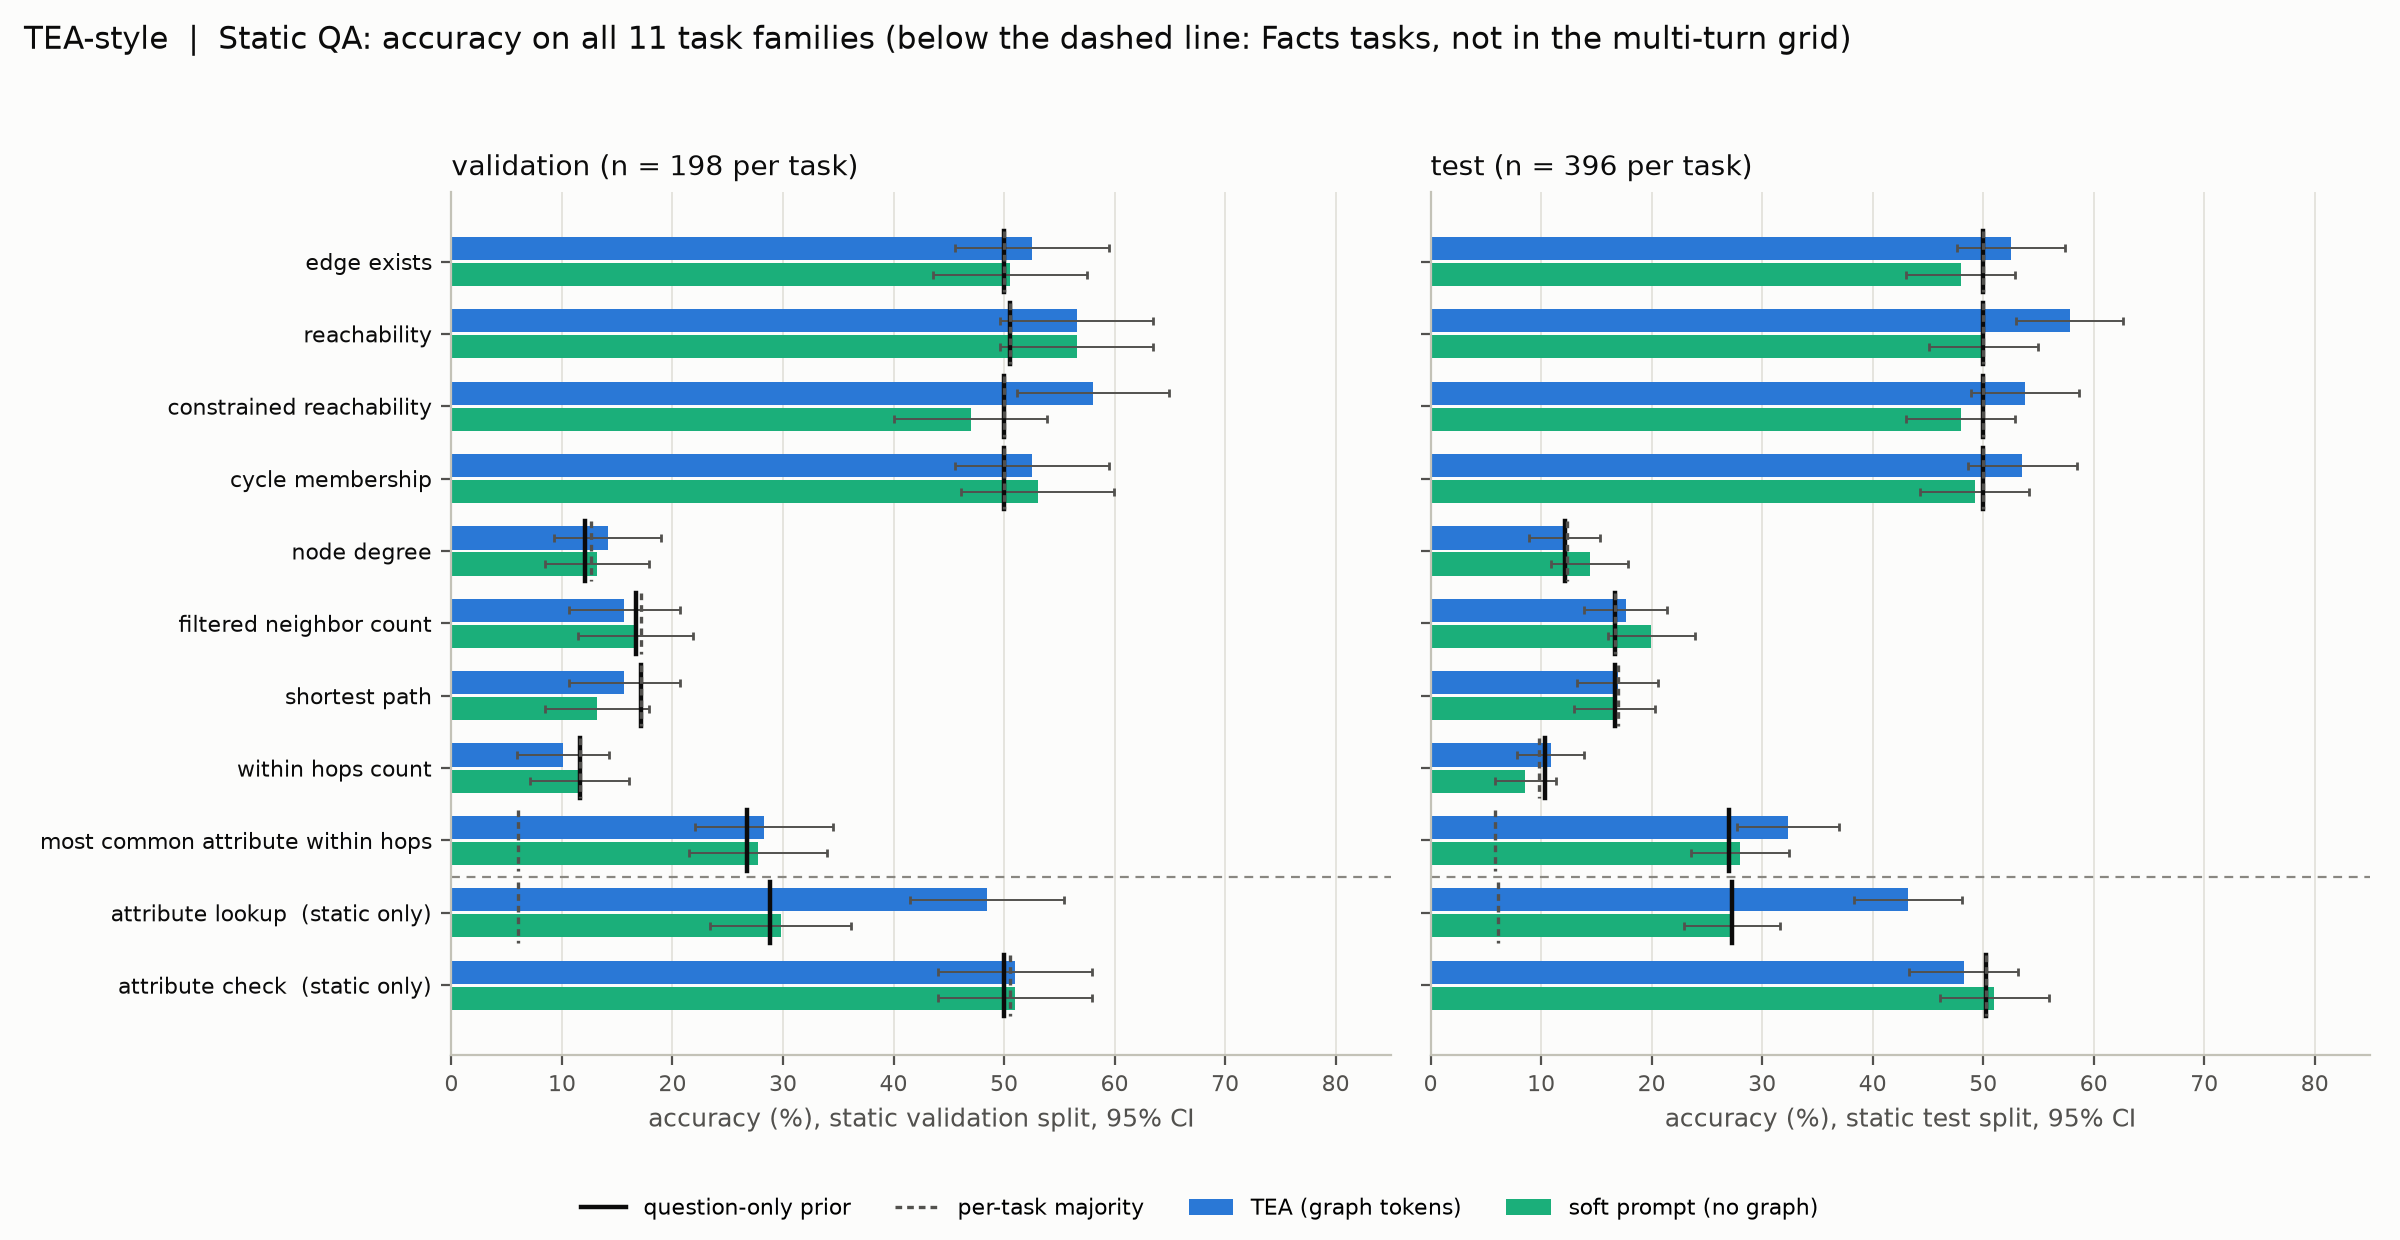
\includegraphics[width=\textwidth]{figures/tea_figA4_static_accuracy_by_task.png}
  \caption{TEA-style static accuracy on all eleven task families, validation (198 items per task)
  and test (396), with the soft prompt for comparison. Solid black ticks mark the question-only
  prior and dashed ticks the per-task majority. Tasks below the dashed line are the Facts tasks,
  which are not part of the multi-turn grid. Error bars are binomial 95\% intervals from one
  seed.}
  \label{fig:static-tasks-tea}
\end{figure*}

\begin{figure*}[t]
  \centering
  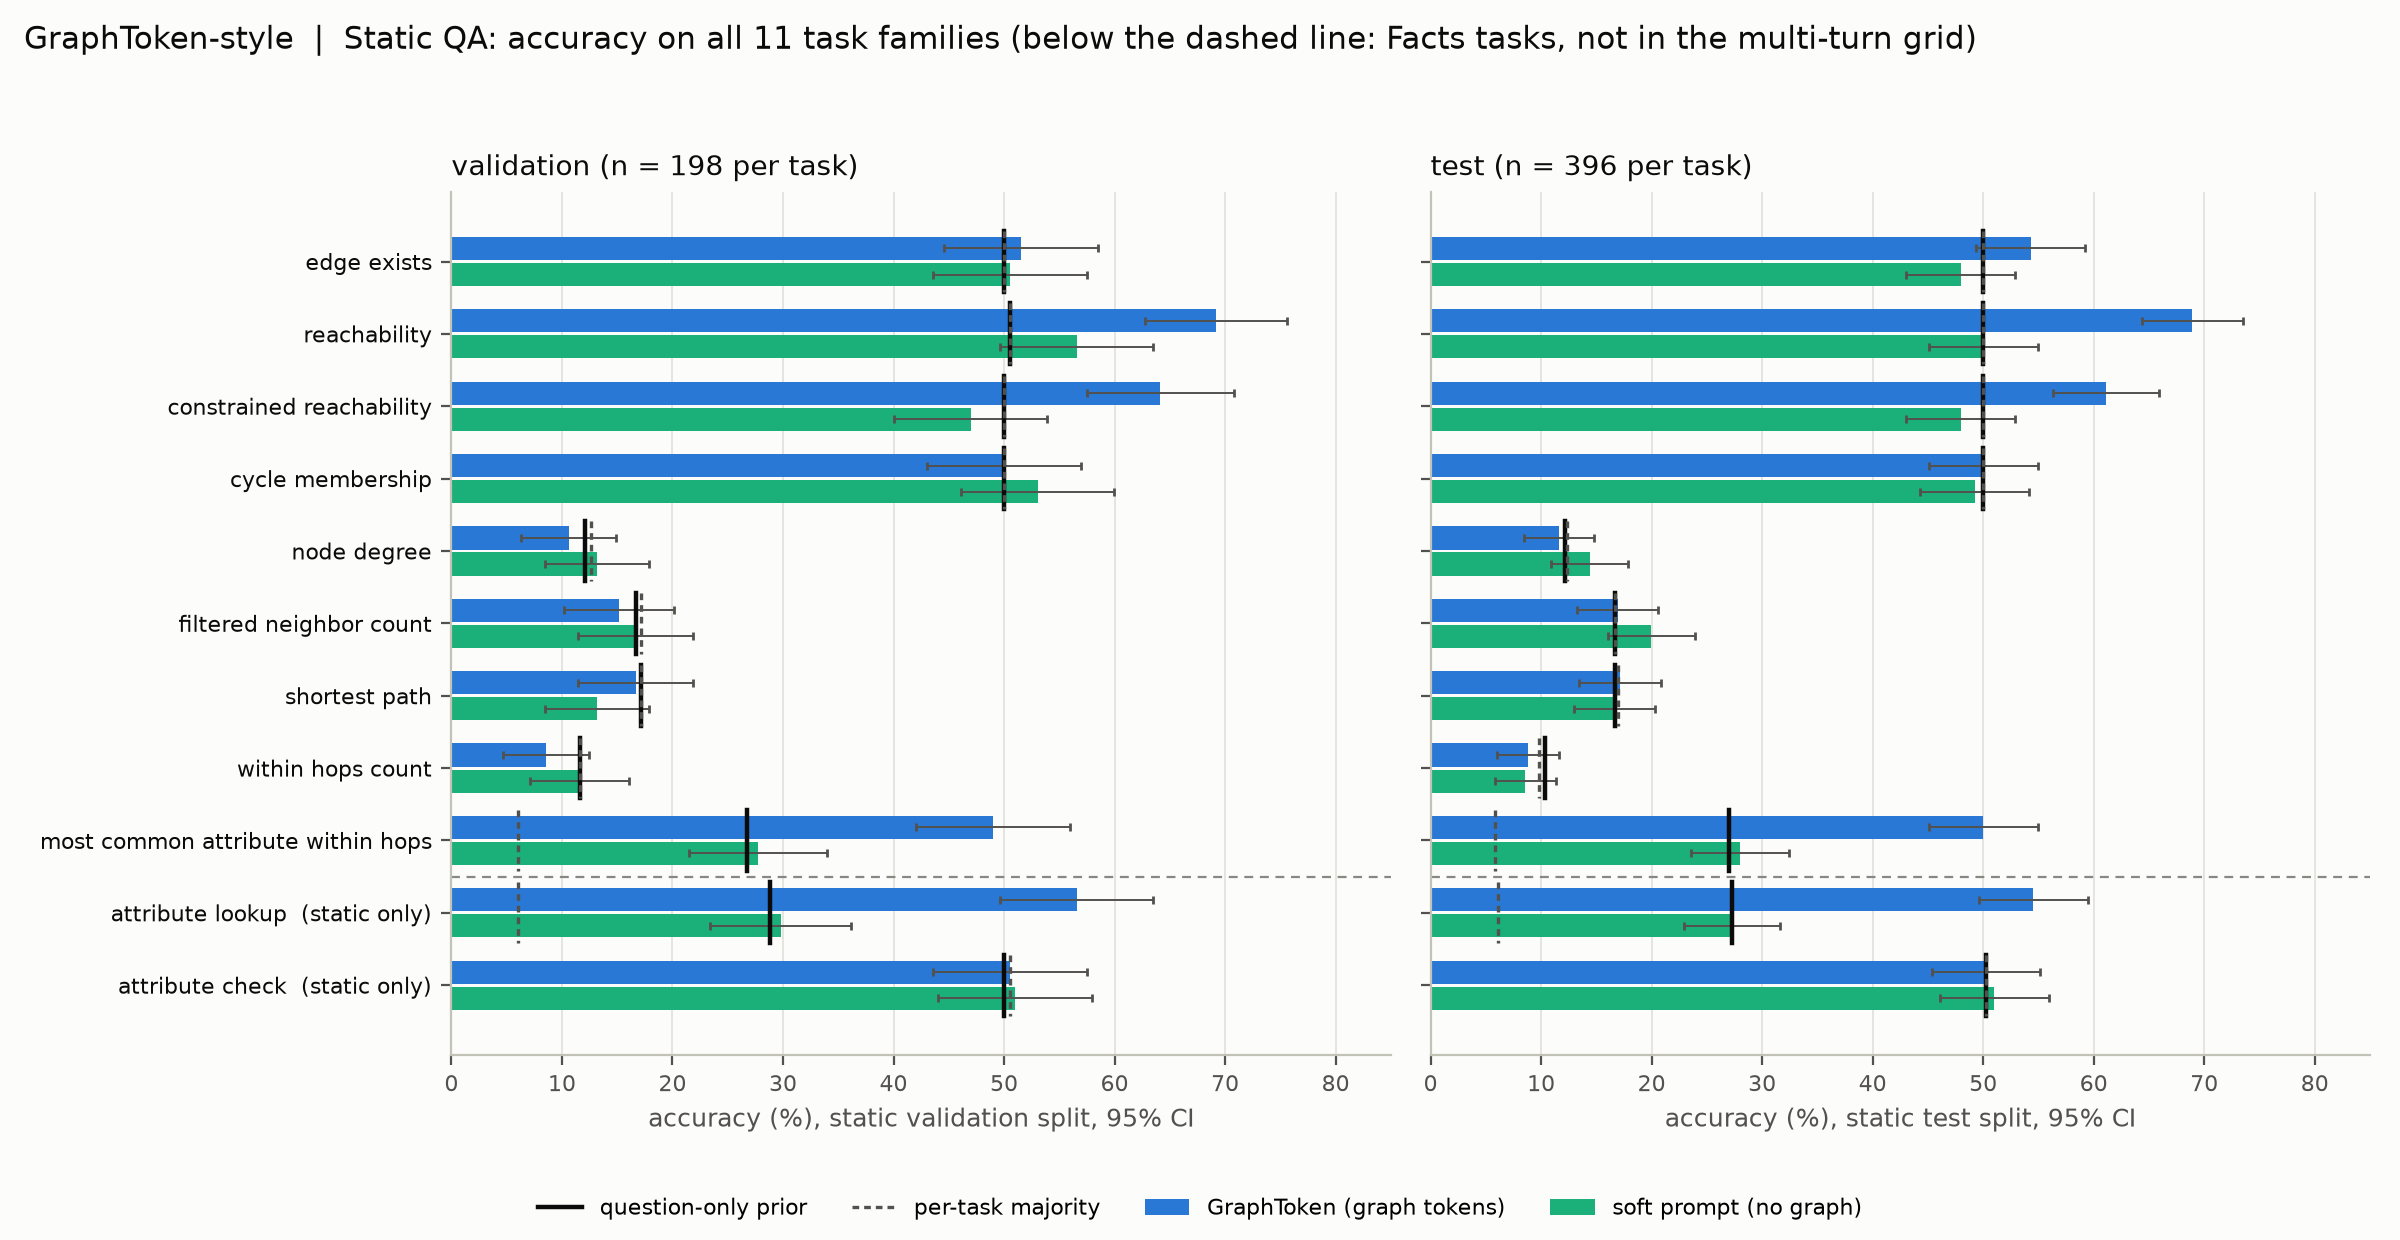
\includegraphics[width=\textwidth]{figures/graphtoken_figA4_static_accuracy_by_task.png}
  \caption{GraphToken-style static accuracy on all eleven task families, laid out as in
  Figure~\ref{fig:static-tasks-tea}. GraphToken-style starts from TEA-style's GNN and, as trained
  here, updates only the projector.}
  \label{fig:static-tasks-gt}
\end{figure*}



\begin{figure*}[p]
\centering
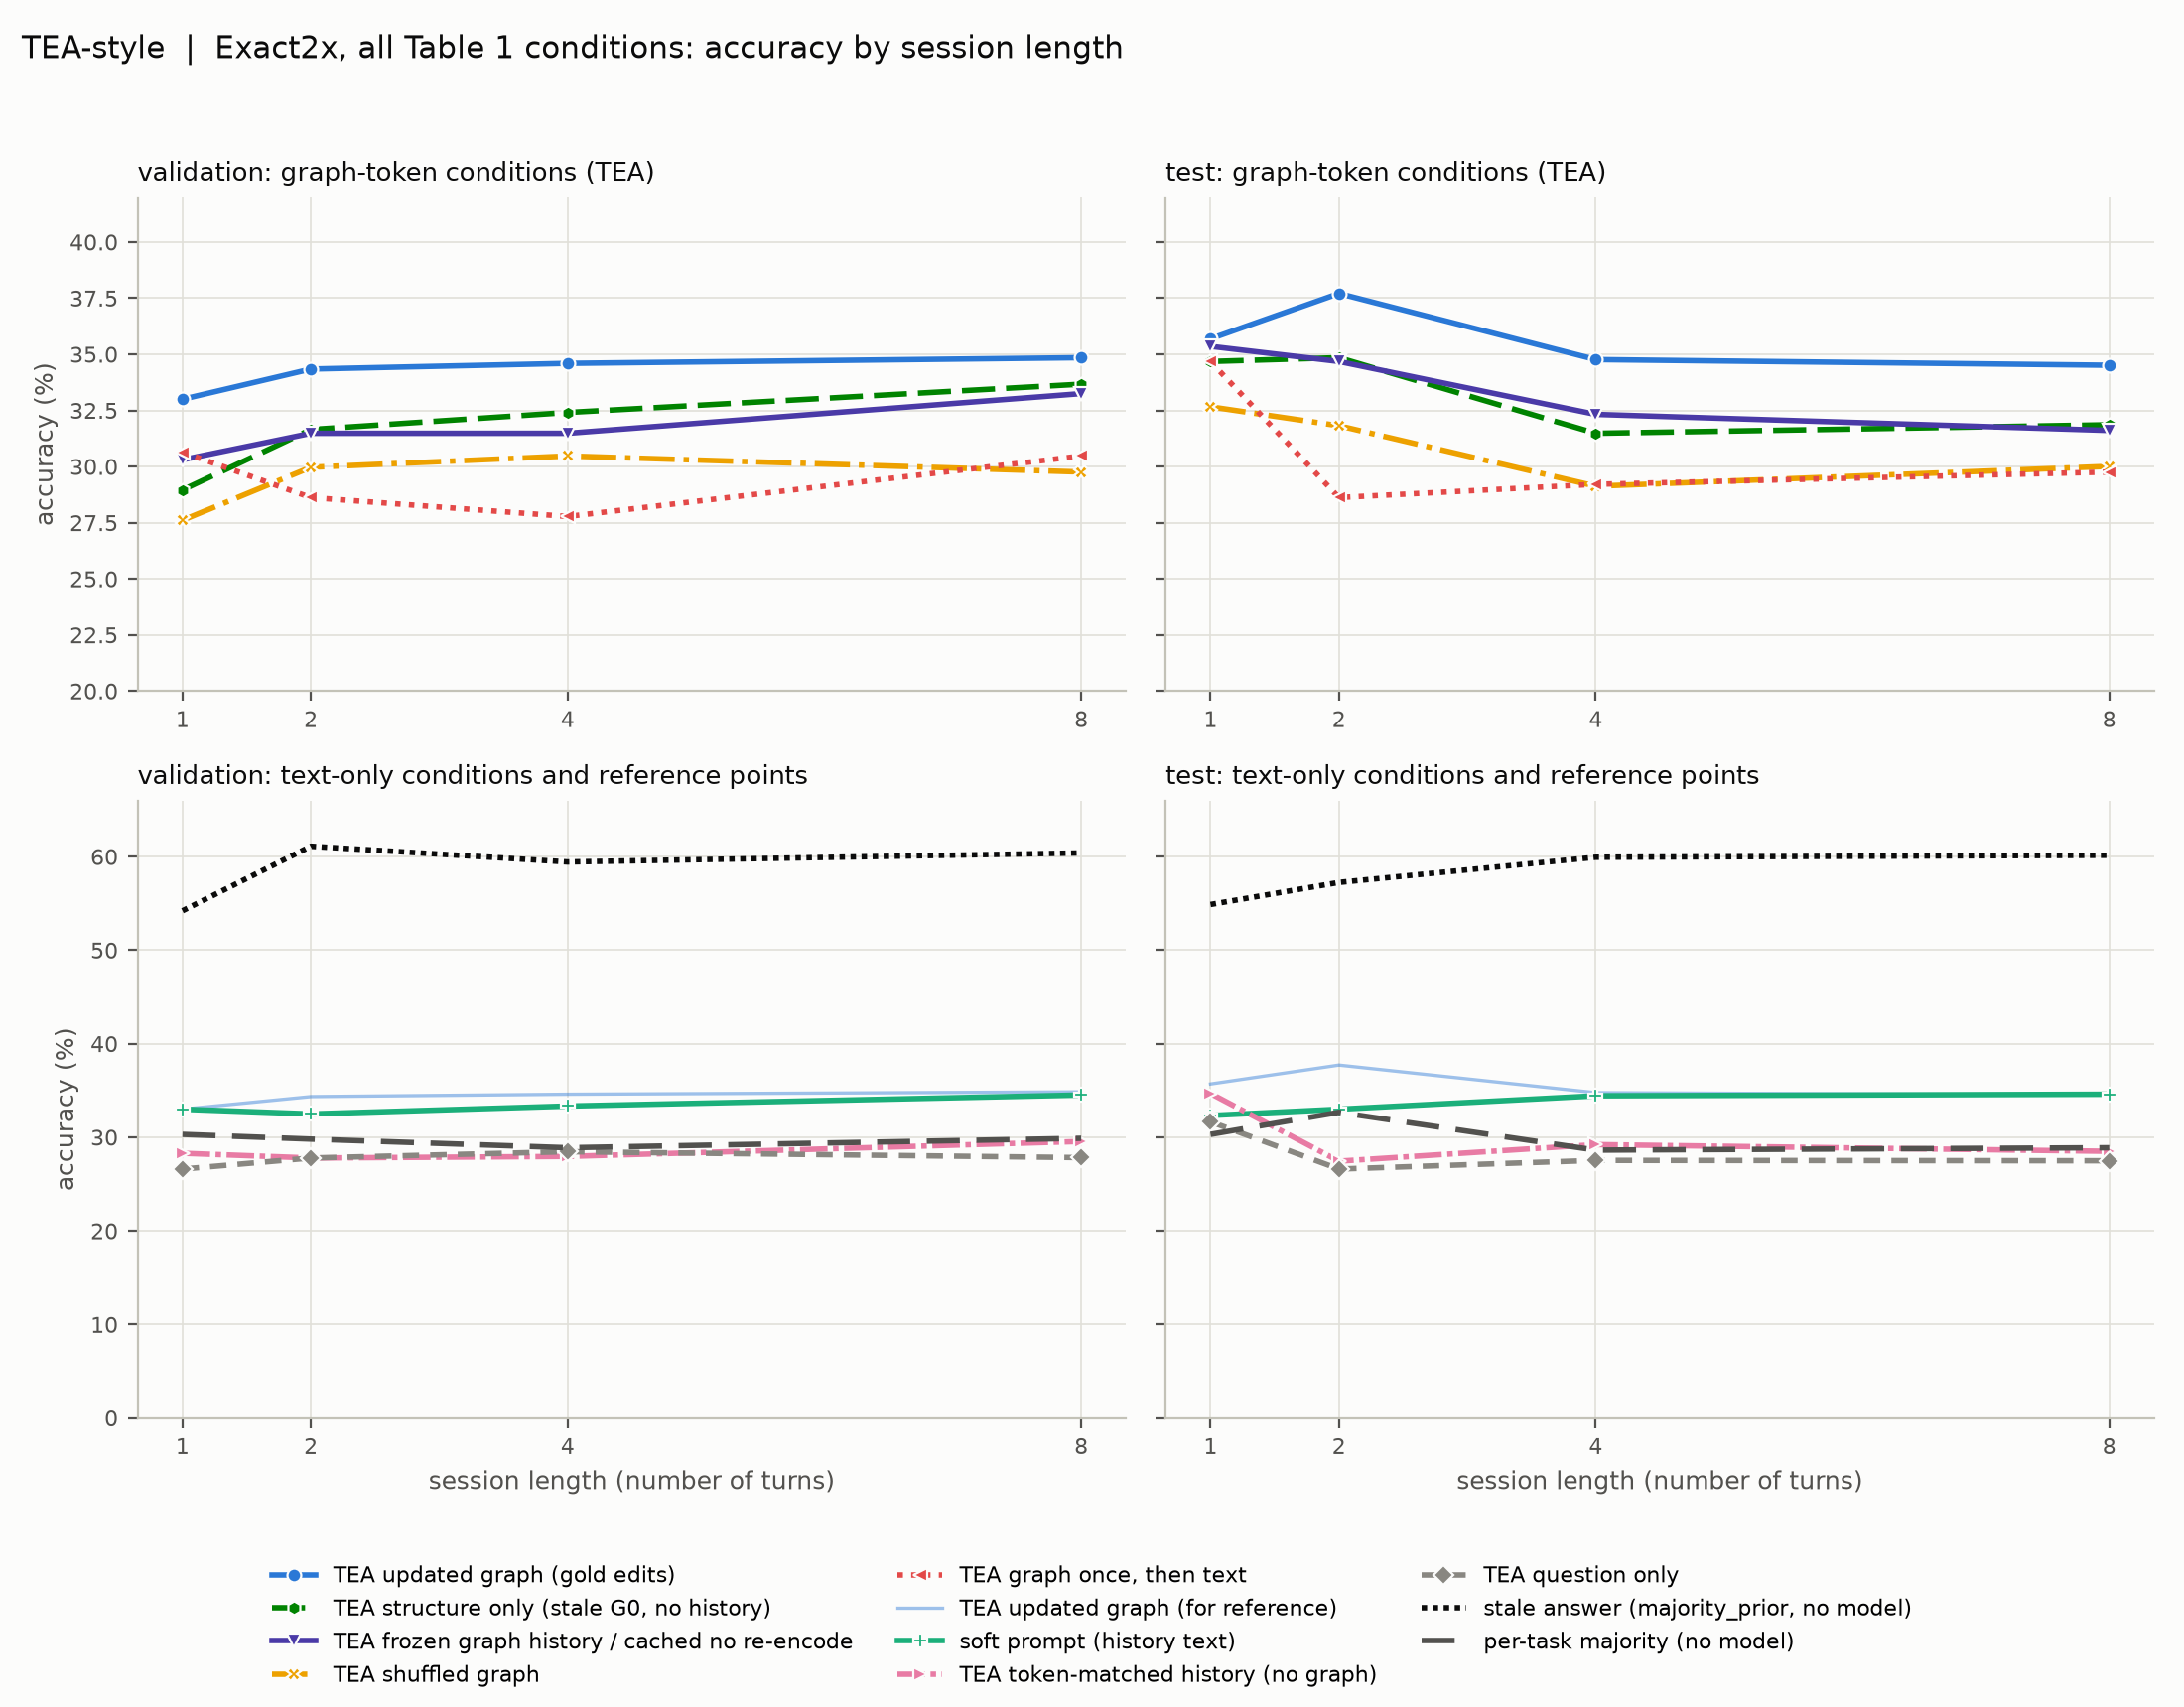
\includegraphics[width=0.9\textwidth,height=0.42\textheight,keepaspectratio]{figures/tea_figA1_all_conditions_by_session_length.png}\\[4pt]
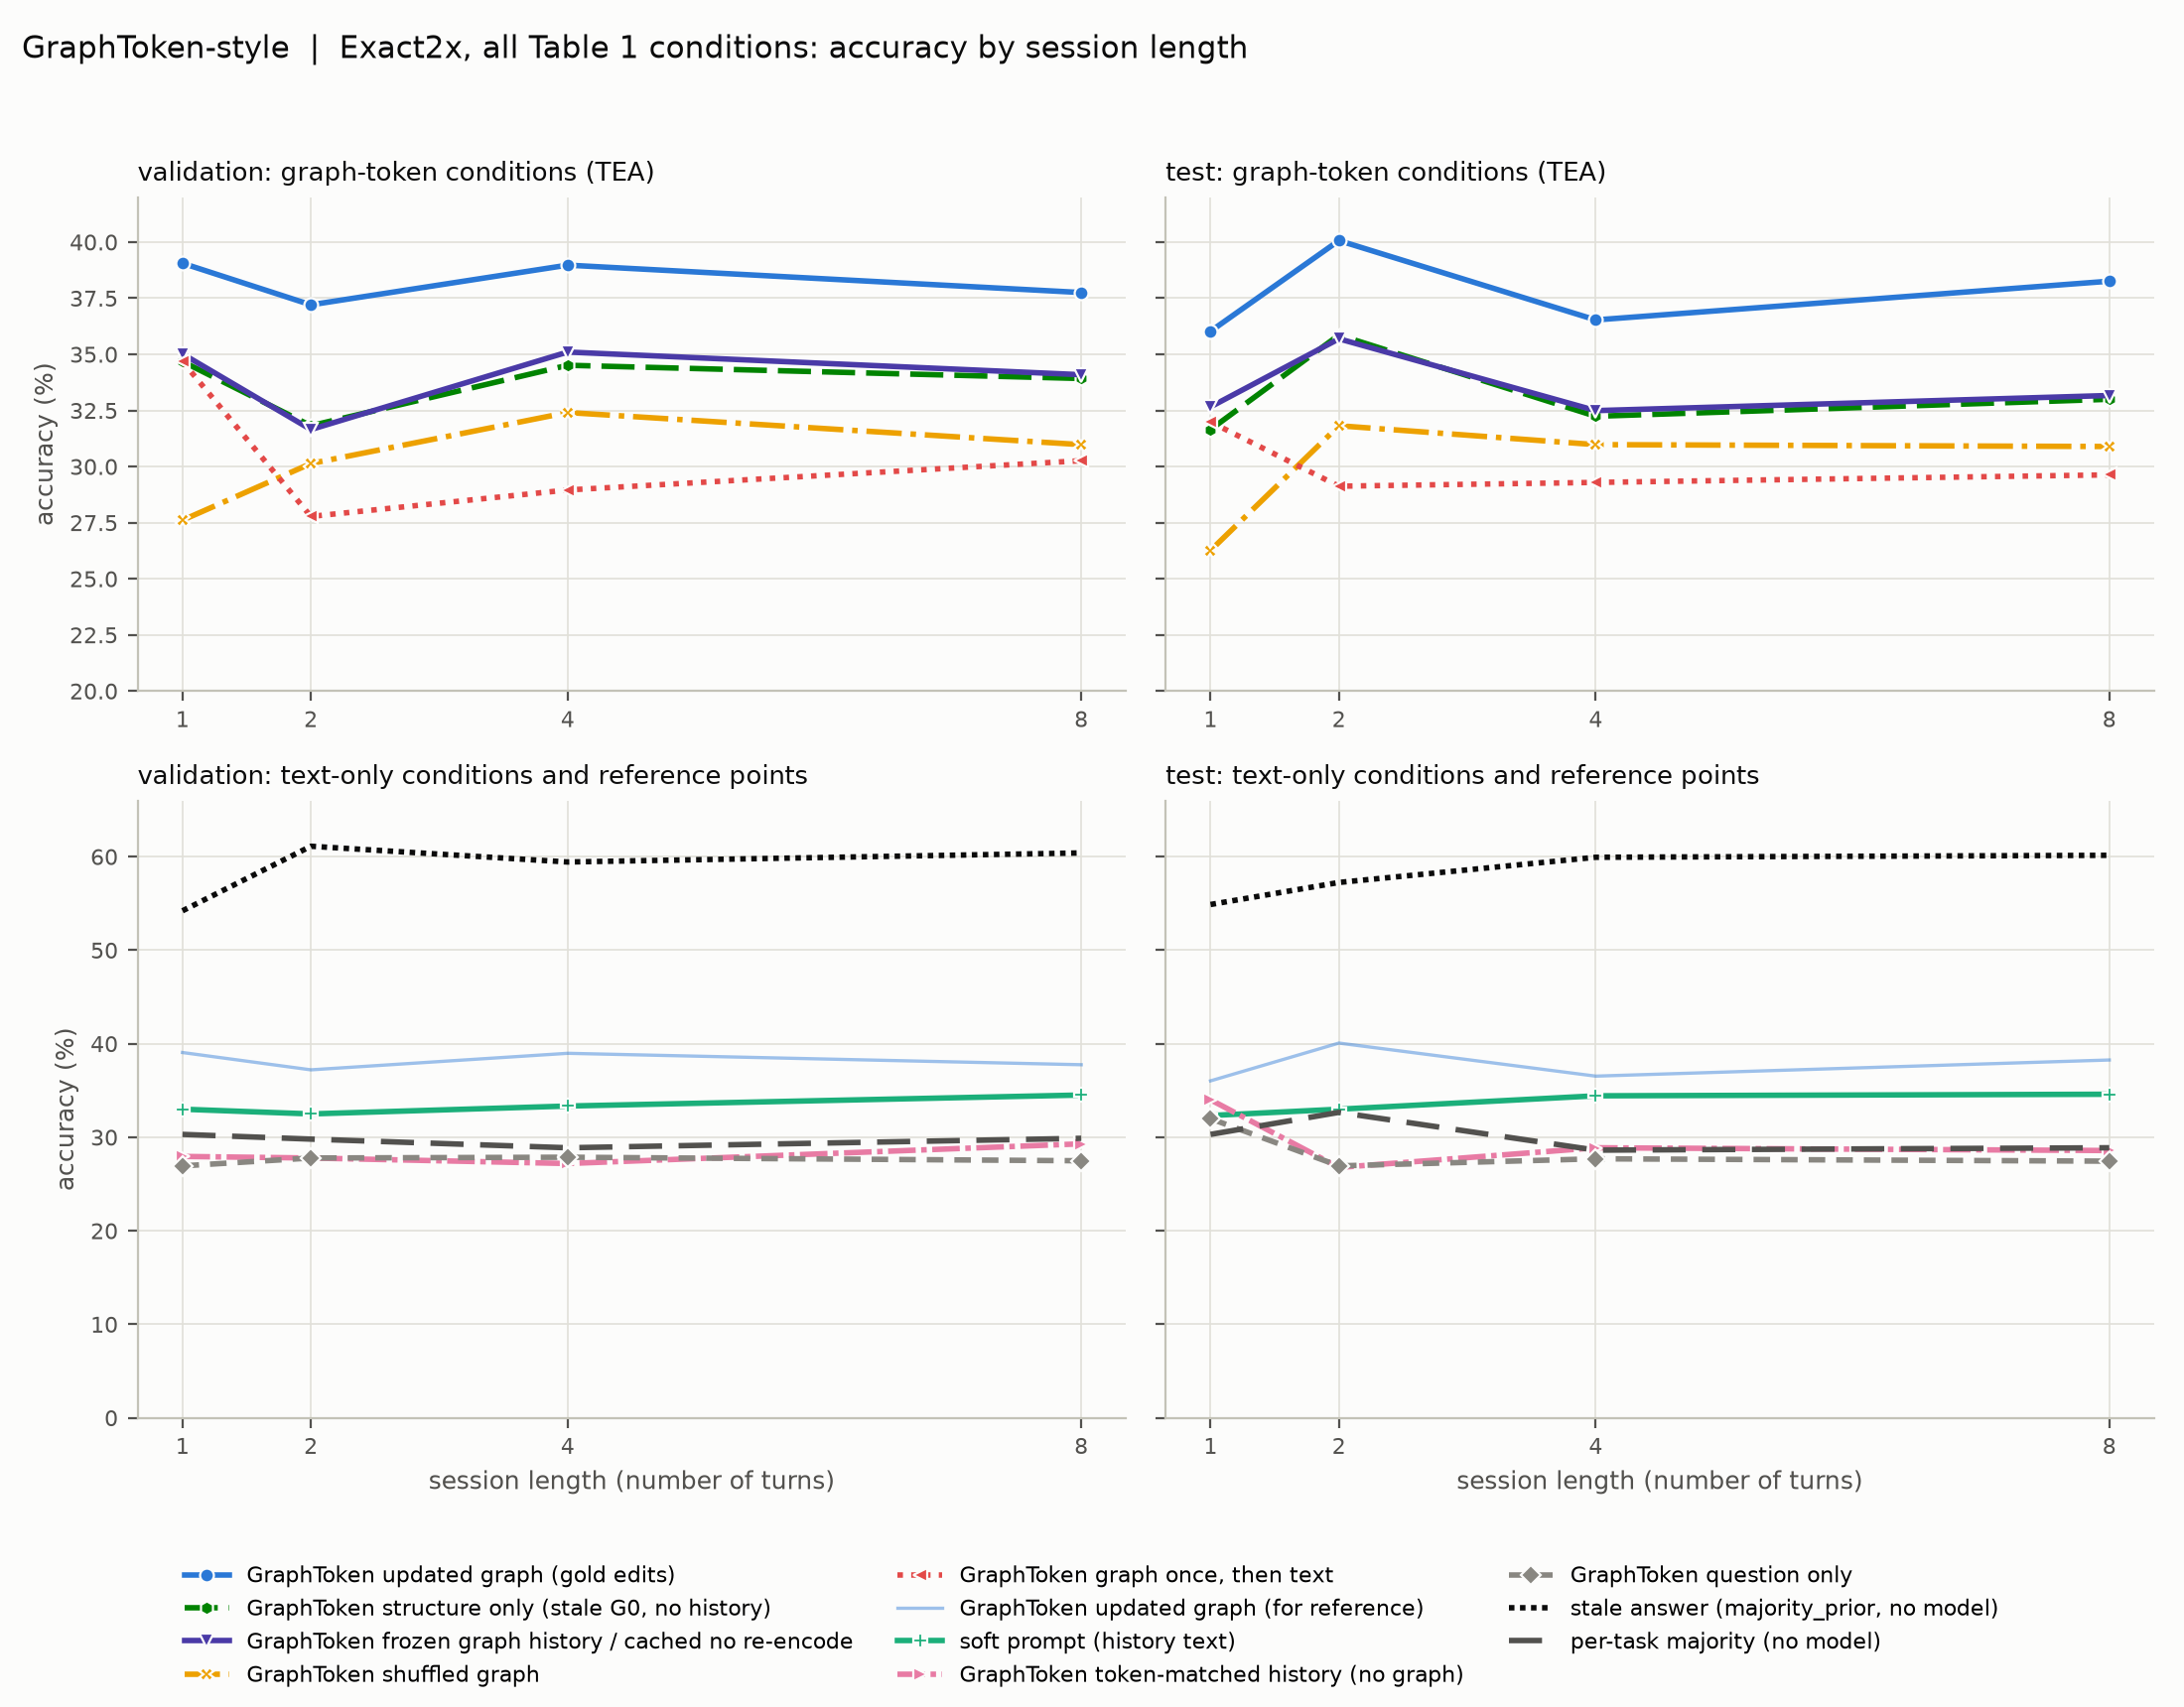
\includegraphics[width=0.9\textwidth,height=0.42\textheight,keepaspectratio]{figures/graphtoken_figA1_all_conditions_by_session_length.png}
\caption{Accuracy by session length for all conditions, TEA-style (top) and GraphToken-style (bottom), validation and test.}
\label{fig:allA1}
\end{figure*}

\begin{figure*}[p]
\centering
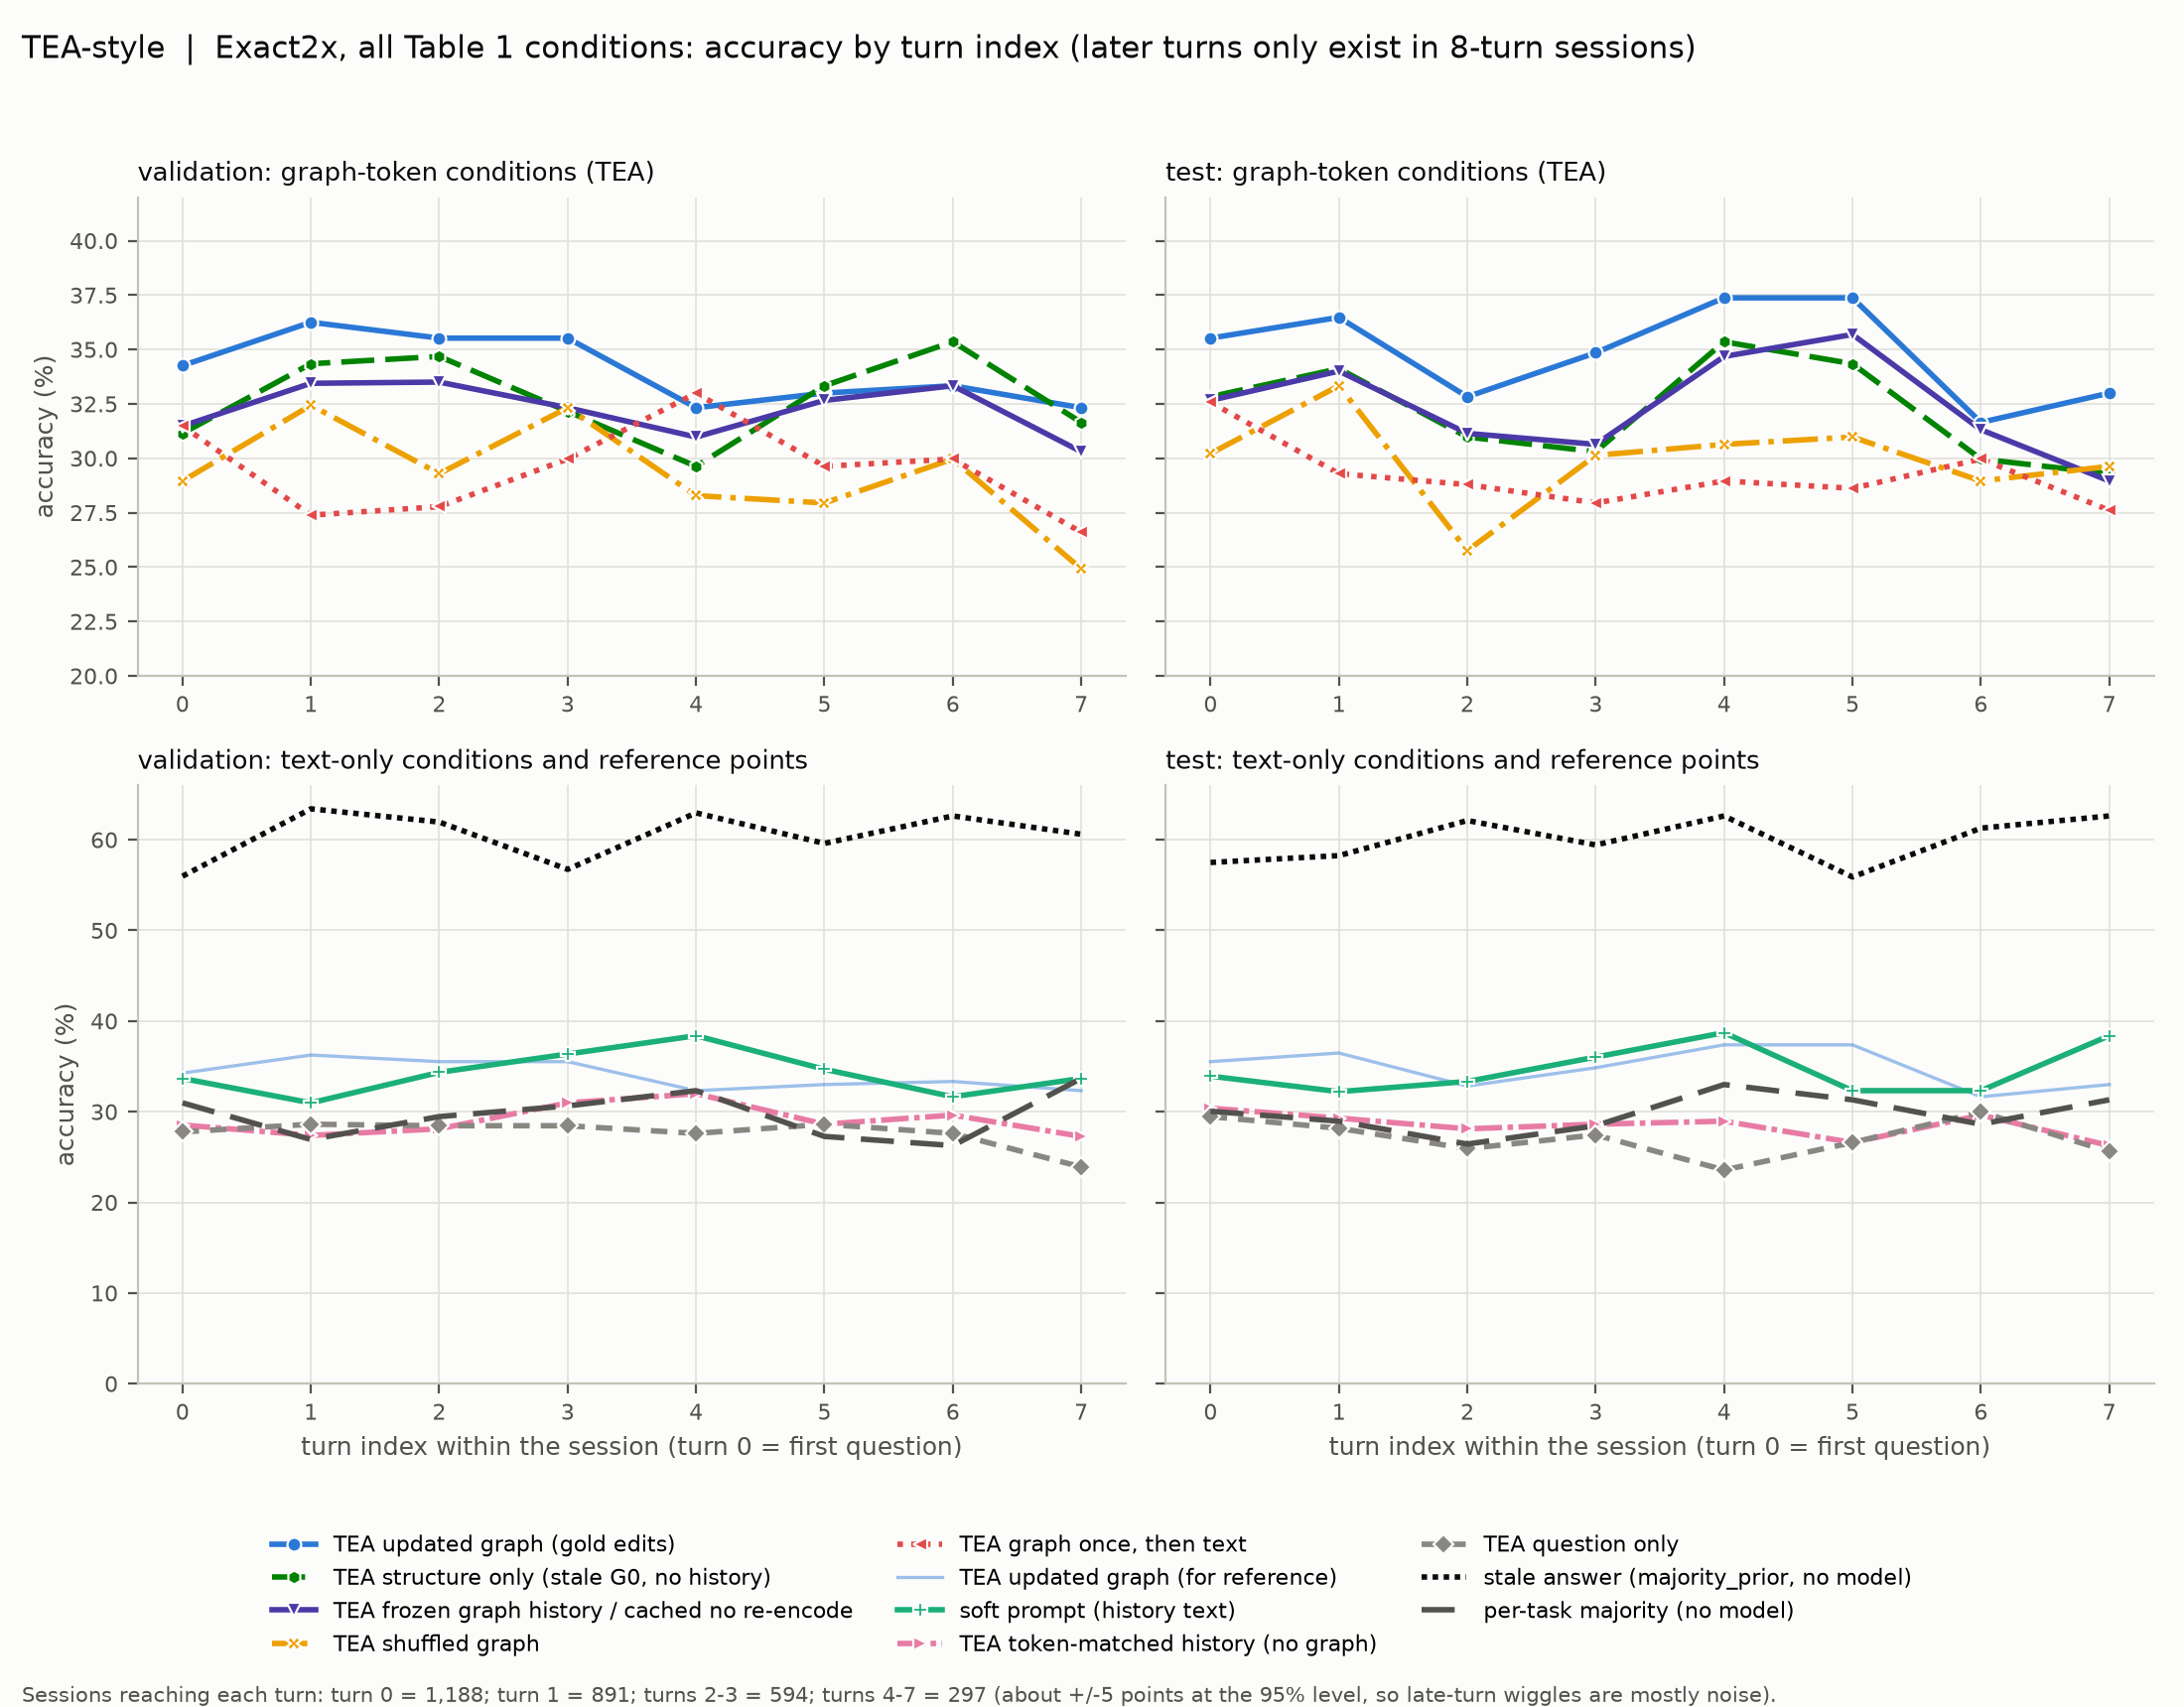
\includegraphics[width=0.9\textwidth,height=0.42\textheight,keepaspectratio]{figures/tea_figA2_all_conditions_by_turn_index.png}\\[4pt]
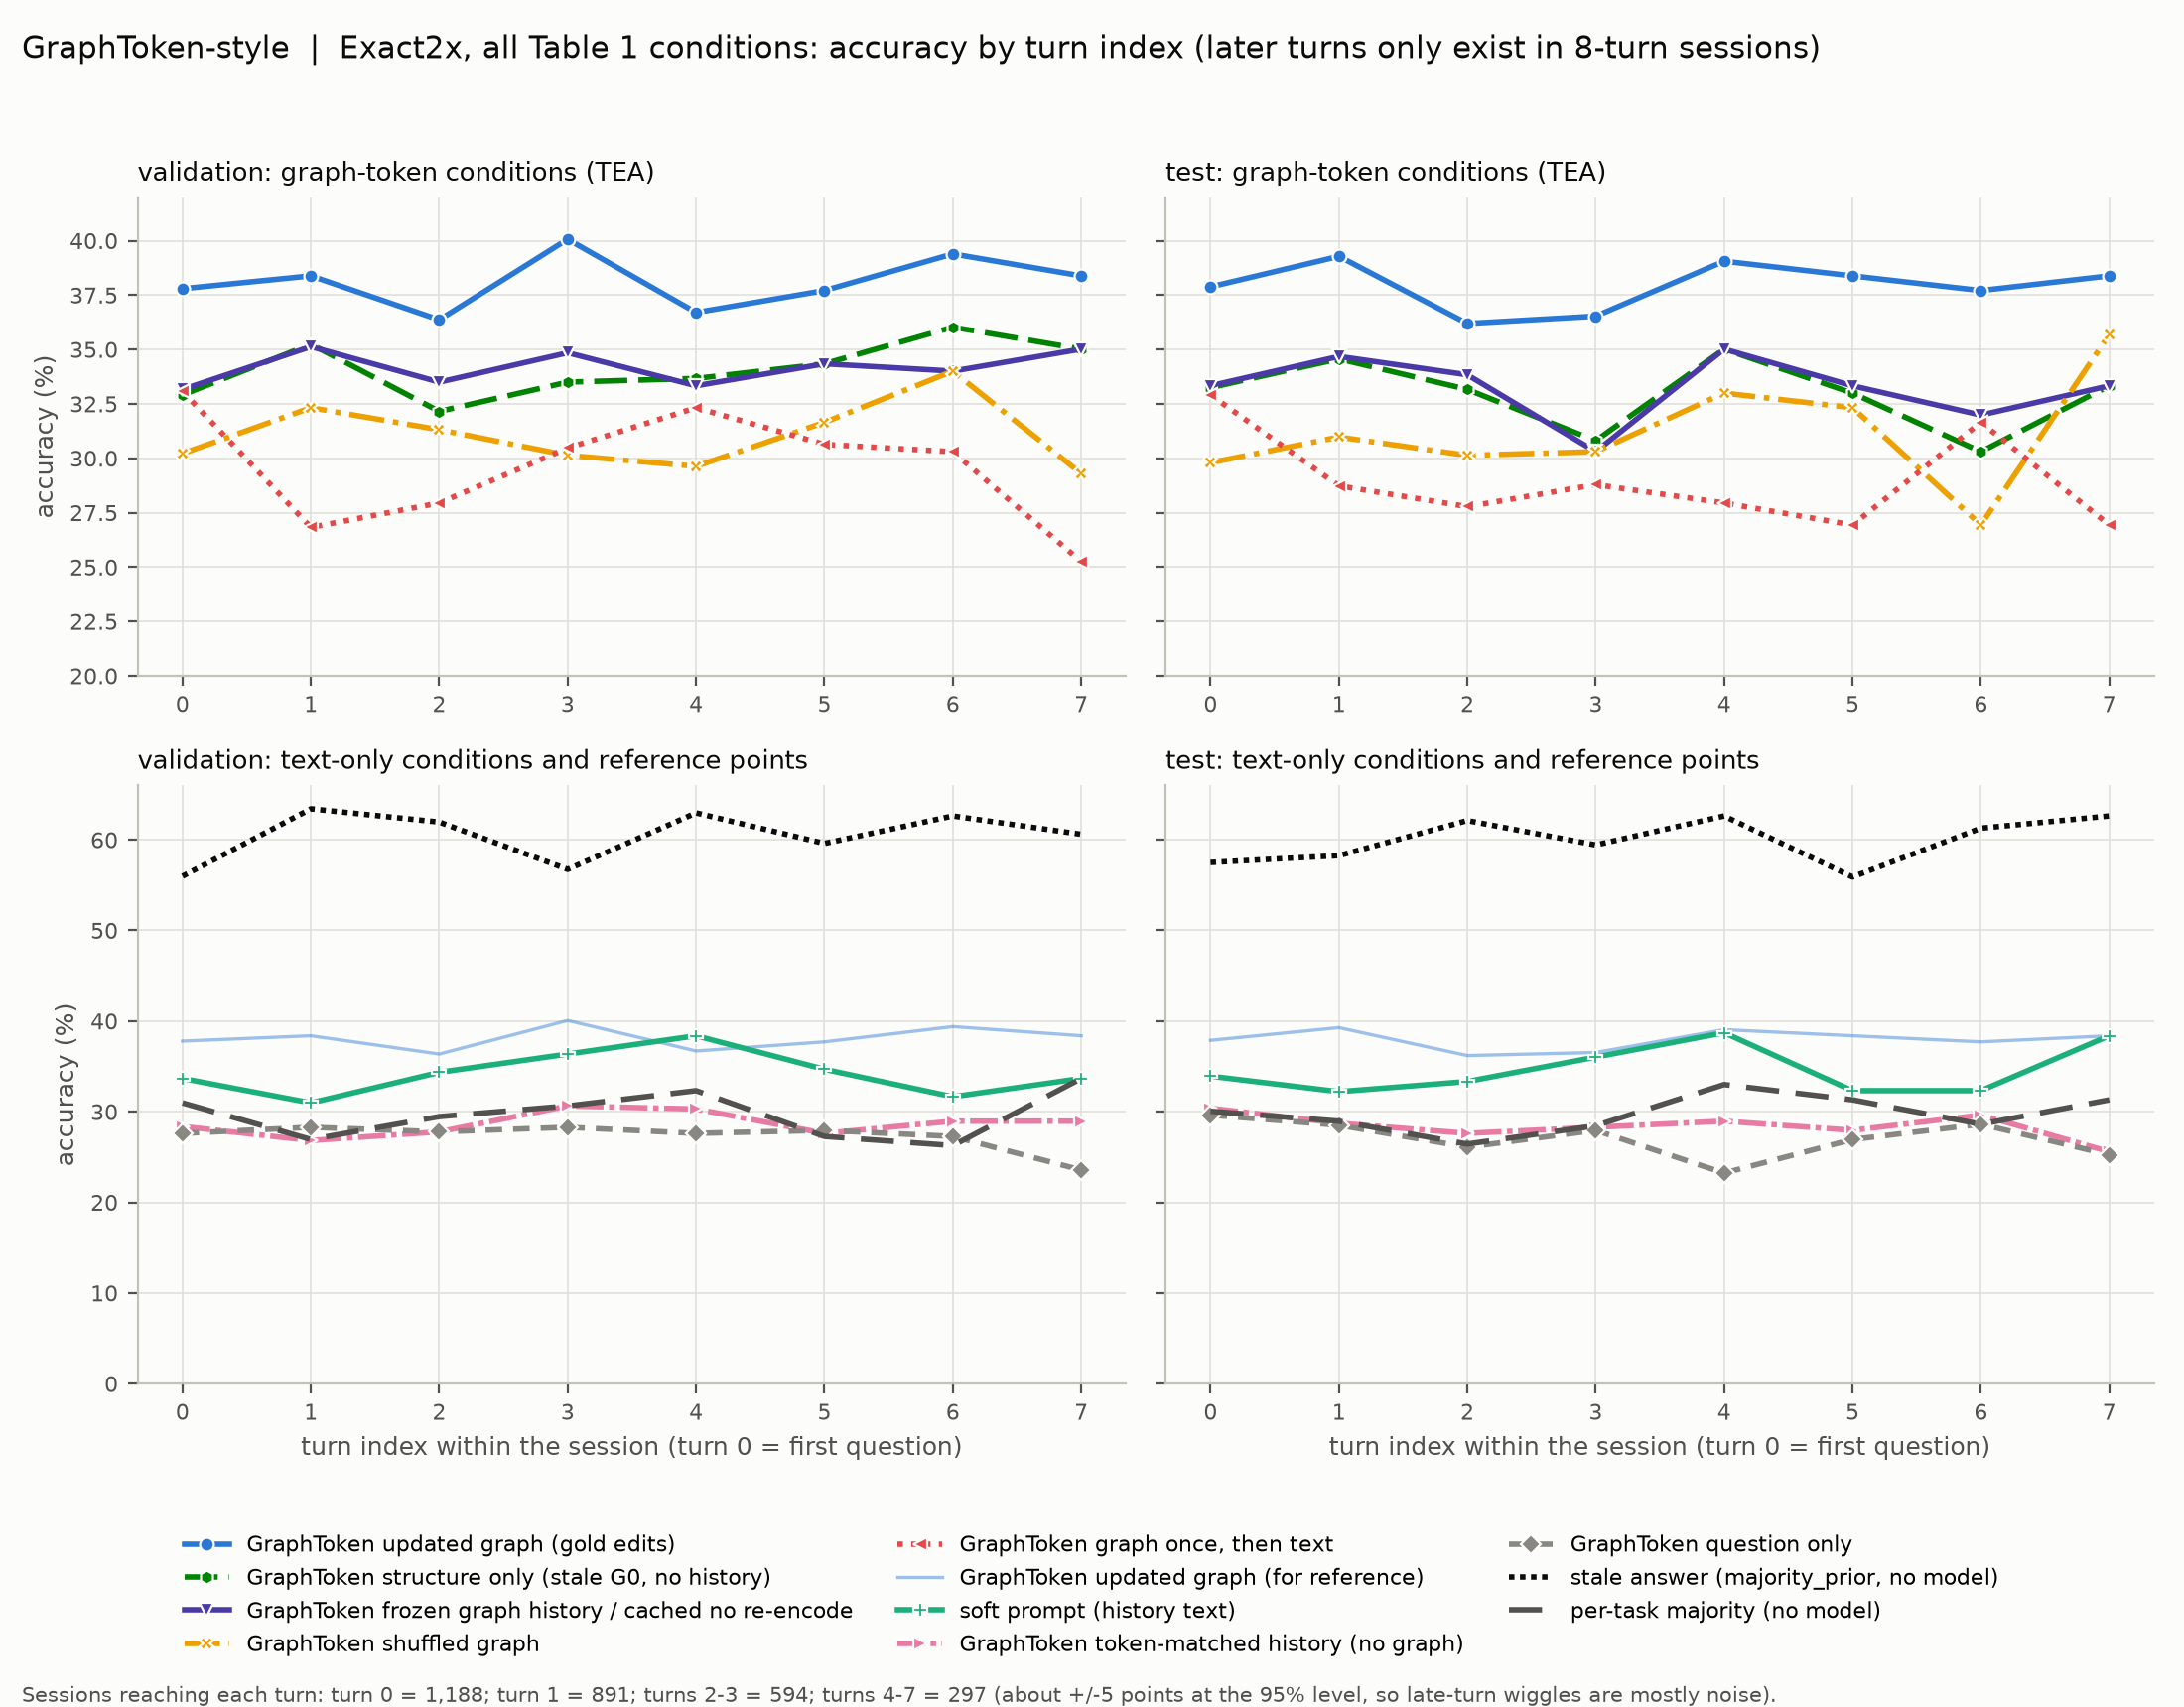
\includegraphics[width=0.9\textwidth,height=0.42\textheight,keepaspectratio]{figures/graphtoken_figA2_all_conditions_by_turn_index.png}
\caption{Accuracy by turn index for all conditions, TEA-style (top) and GraphToken-style (bottom), validation and test. Later turns only occur in 8-turn sessions.}
\label{fig:allA2}
\end{figure*}

\begin{figure*}[p]
\centering
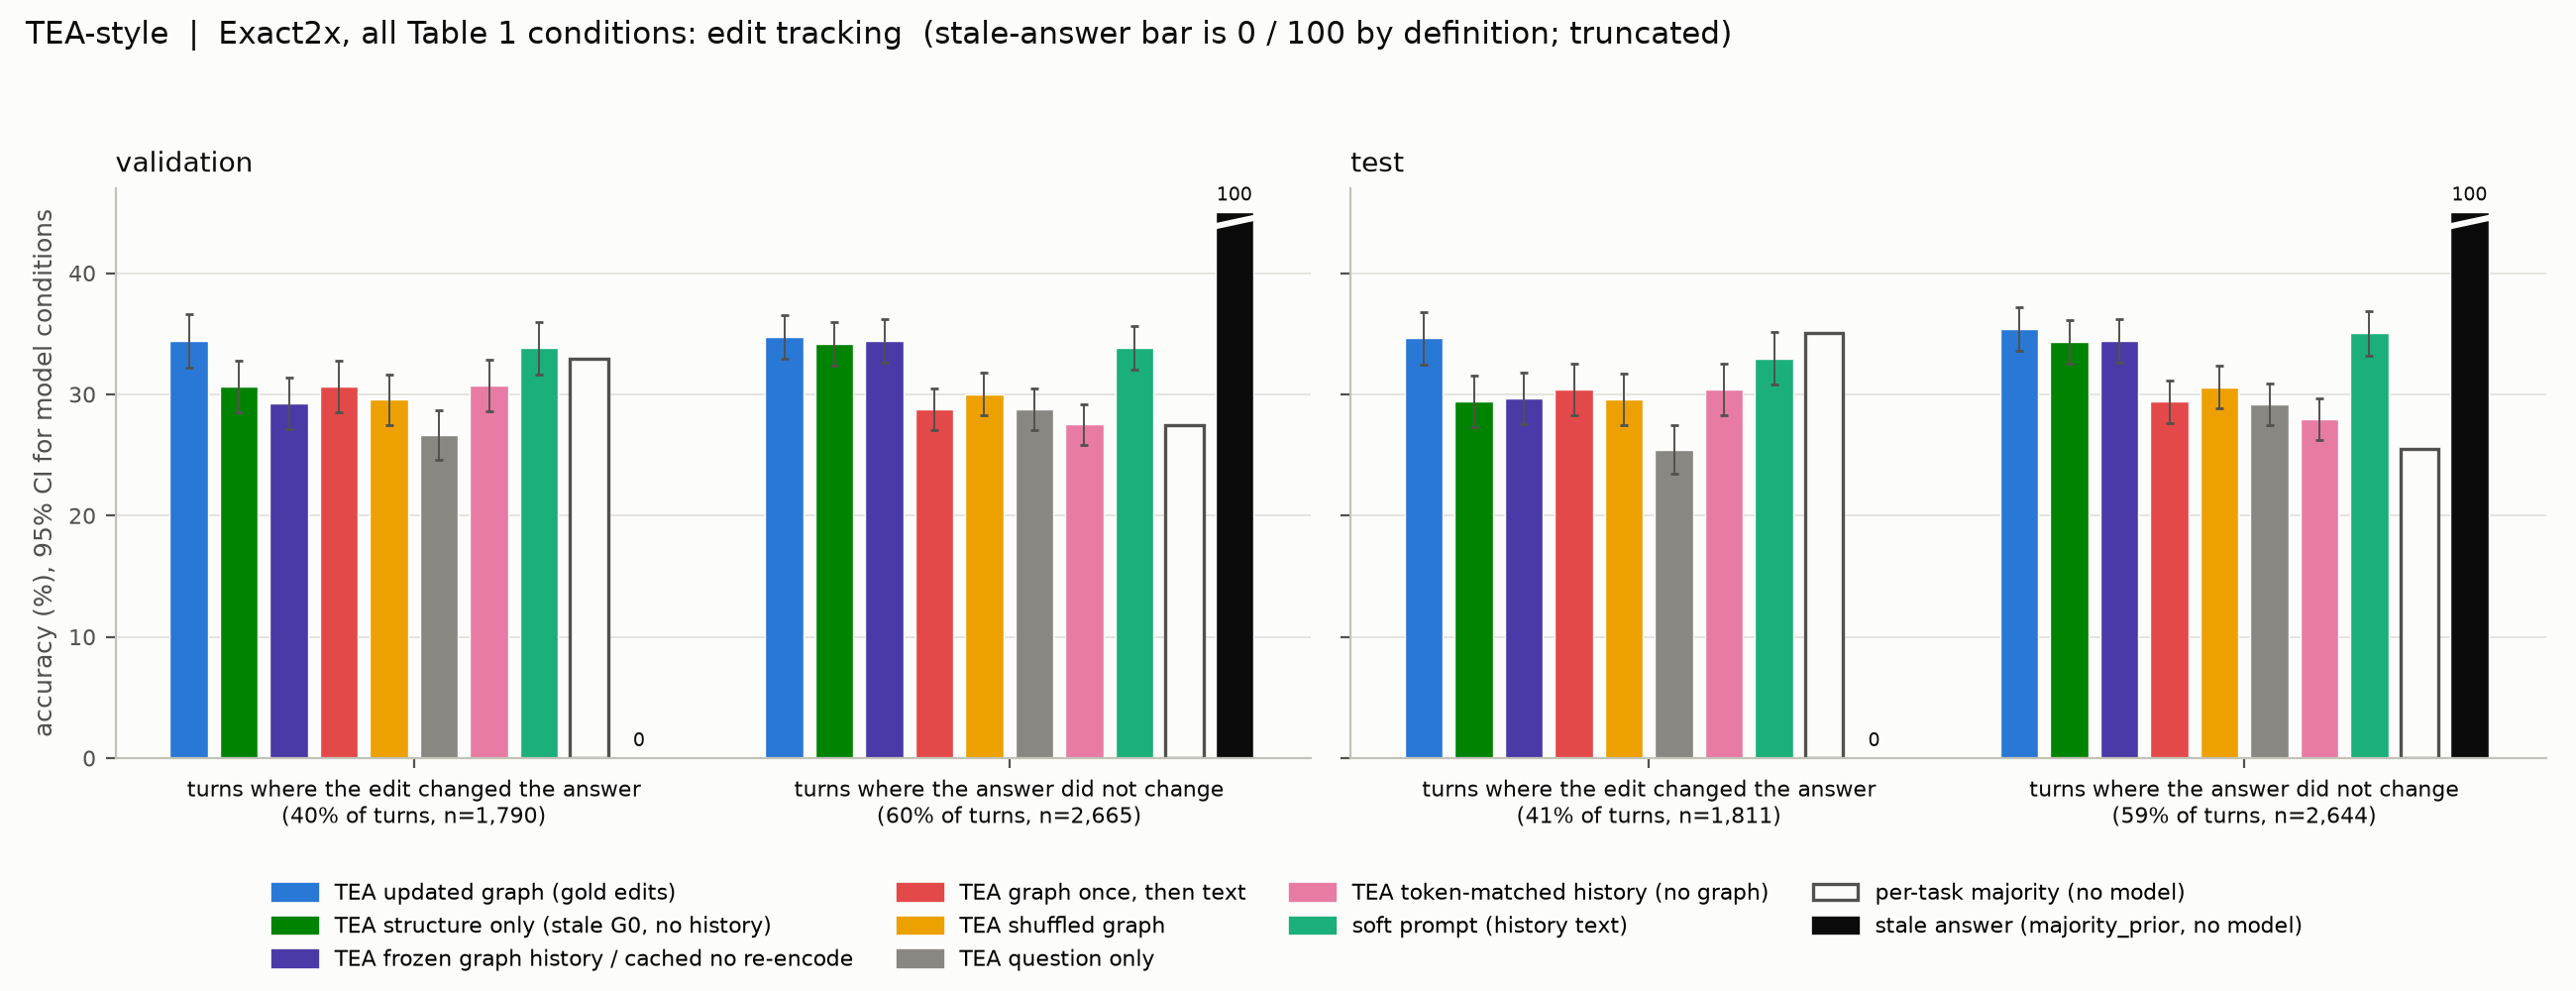
\includegraphics[width=0.9\textwidth,height=0.42\textheight,keepaspectratio]{figures/tea_figA3_all_conditions_edit_tracking.png}\\[4pt]
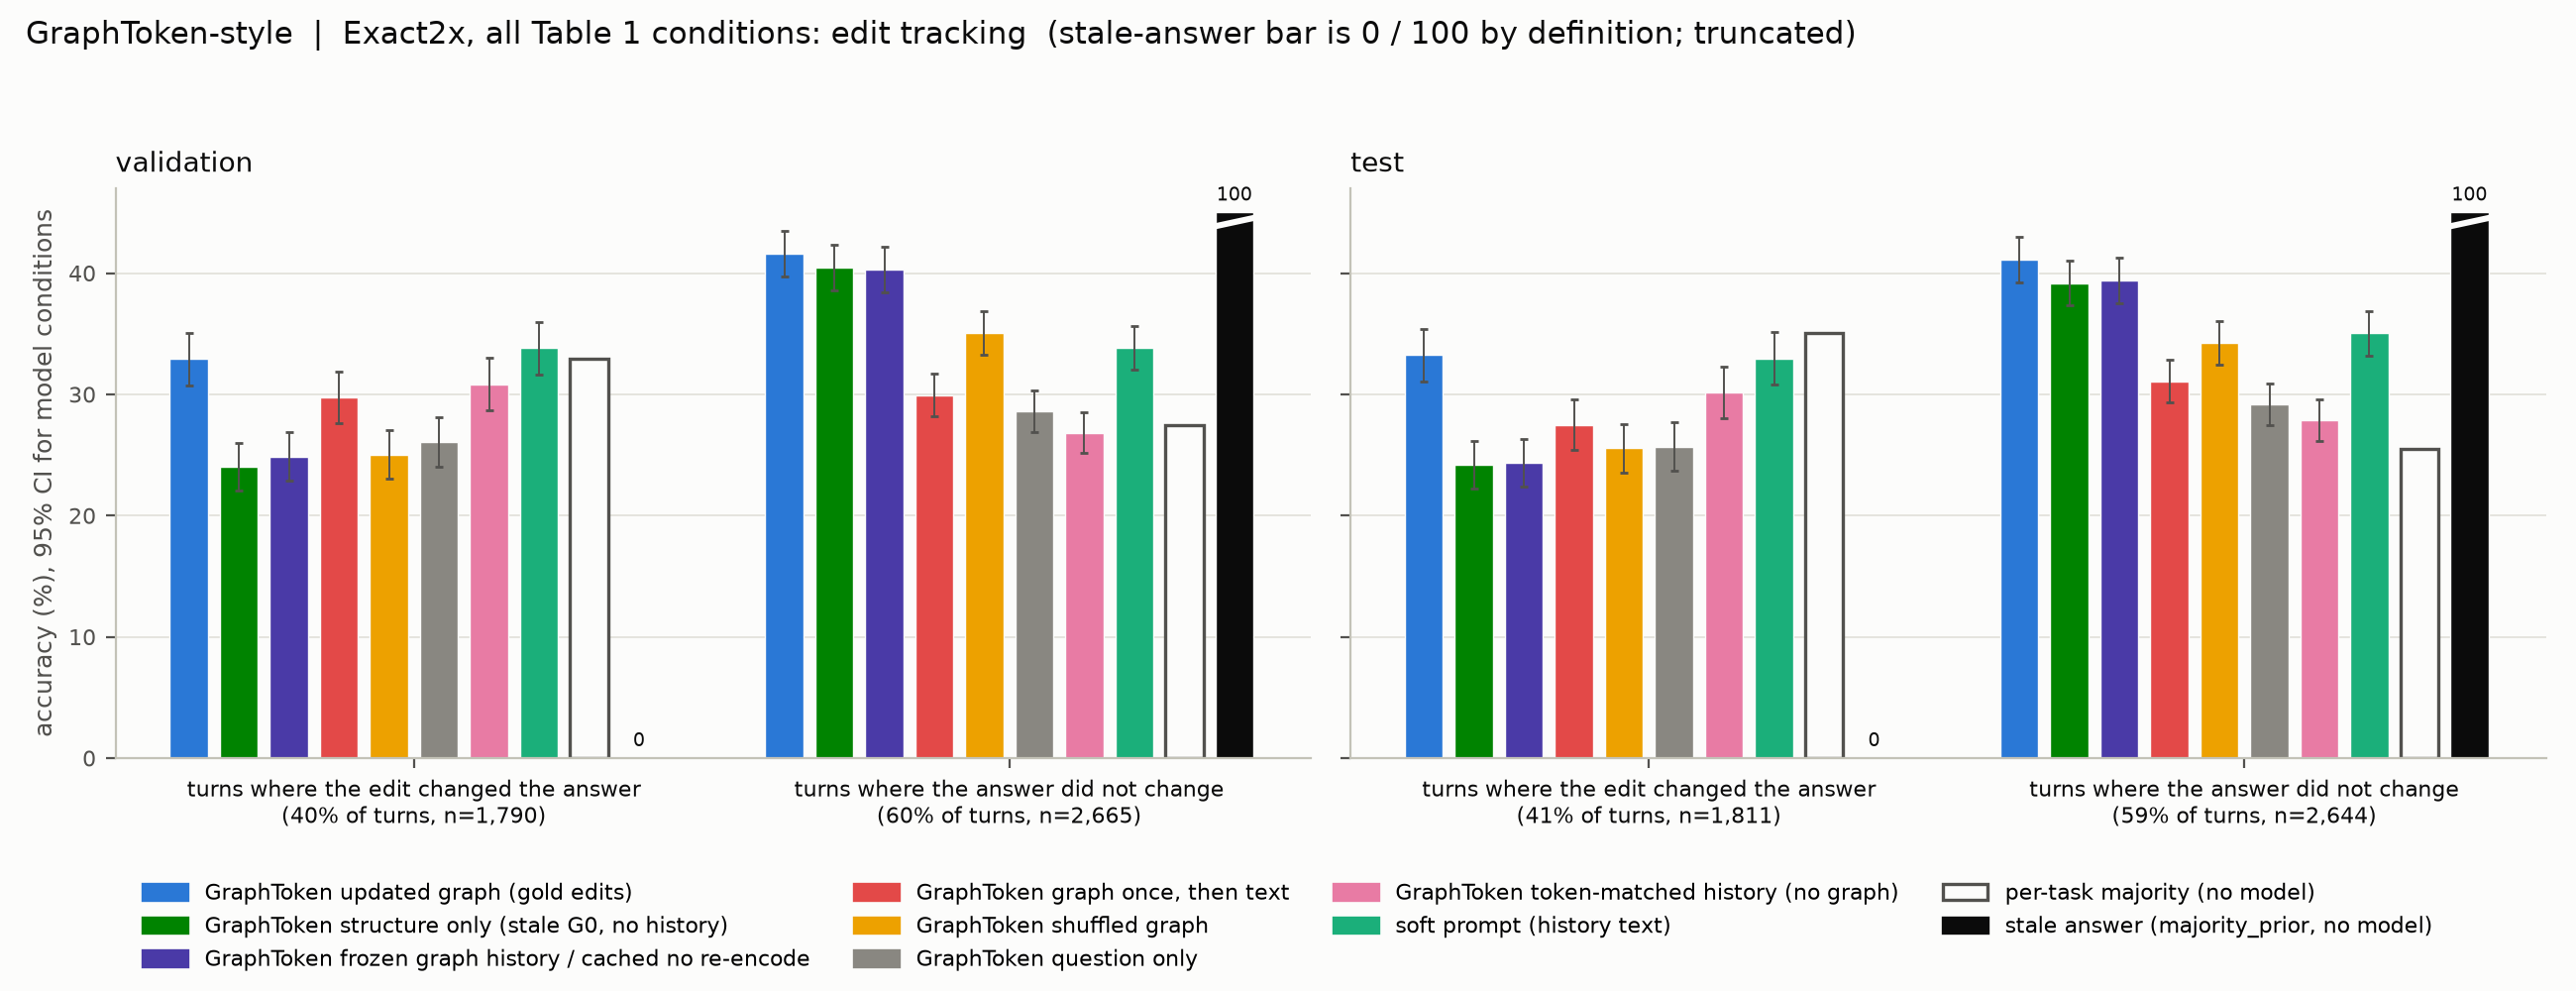
\includegraphics[width=0.9\textwidth,height=0.42\textheight,keepaspectratio]{figures/graphtoken_figA3_all_conditions_edit_tracking.png}
\caption{Accuracy on answer-changing and unchanged turns for all conditions, TEA-style (top) and GraphToken-style (bottom), validation and test. The stale-answer bar is truncated.}
\label{fig:allA3}
\end{figure*}

\section{Hyperparameters}
\label{app:hparams}

\begin{table}[t]
\centering
\small
\resizebox{\linewidth}{!}{%
\begin{tabular}{@{}ll@{}}
\toprule
\textbf{Item} & \textbf{Value} \\
\midrule
LLM & Llama-3.1-8B-Instruct, bf16, frozen \\
Node features & \texttt{bert-base-uncased}, 768-d, frozen \\
GNN & GraphSAGE 768/1024/1024, 3 layers, mean, dropout 0.5 \\
Projector & $3087\to10\times4096$, linear \\
InfoNCE & 10 epochs, 8 graphs/batch, lr $10^{-3}$, $\tau{=}0.07$ \\
Projector training & AdamW, lr $10^{-3}$, wd $10^{-4}$, eff.\ batch 24 \\
Epochs & 5 for all models \\
\bottomrule
\end{tabular}%
}
\caption{Key hyperparameters.}
\label{tab:hparams}
\end{table}

\end{document}